\documentclass{report}
\usepackage[spanish]{babel}
\usepackage[utf8]{inputenc}
\usepackage{amsmath, array}
\usepackage{amssymb}
\usepackage{tabularx}
\usepackage{minted}
\RecustomVerbatimEnvironment{Verbatim}{BVerbatim}{}
\usepackage{cite}
\usepackage{graphicx}
\usepackage{graphbox}
\usepackage{color}
\usepackage{float}
\usepackage{subfigure}
\usepackage{amsfonts}
\usepackage[section]{placeins}
\usepackage{hyperref}
\usepackage{blindtext}
\usepackage{scrextend}
\addtokomafont{labelinglabel}{\sffamily}
\hypersetup{
     colorlinks=true,
     citecolor=black,
     filecolor=black,
     linkcolor=black,
     urlcolor=blue
}
\date{}
\setcounter{secnumdepth}{3} % Add number to subsubsections
\usepackage{framed}

% counter used for definitions. Every time you want to add a definition, use
% \stepcounter{definitionsCounter} before the definition
\newcounter{definitionsCounter}

\begin{document}
    %Nombre templetizado para poder cambiarlo fácil hasta tenerlo definido
    \newcommand{\nombreTesis}{Framework de Sincronización de Tareas Coordinado
    por Redes de Petri}
    %Nombre templetizada por si lo tenemos que cambiar
    \newcommand{\nombreFramework}{Baboon}
    %Nombre del monitor templetizado
    \newcommand{\javapetriconcurrencymonitor}{Java Petri Concurrency Monitor }

    \title{\nombreTesis}
    \author{Ariel Iván Rabinovich \\ \href{mailto:airabinovich@gmail.com}{airabinovich@gmail.com}
        \and Juan José Arce Giacobbe \\ \href{mailto:juanjo.arce7546@gmail.com}{juanjo.arce7456@gmail.com}}
    \graphicspath{ {resources/images/} }
    
    \maketitle
    
    \tableofcontents
    
    \listoffigures
    \listoftables
    
    \setcounter{definitionsCounter}{0}
    
    \part{Marco Teórico}
        \chapter{Introducción}
            \section*{Introducción}

La finalidad del marco teórico es introducir al lector en los conceptos
necesarios para la comprensión del desarrollo de este proyecto integrador.
Los temas aquí desarrollados y/o referidos son necesarios para alcanzar los
objetivos antes propuestos.

        \chapter{Modelos}
            \section{Autómatas o Máquinas de Estado}

Existen muchas formas de modelar el comportamiento de los sistemas, y el uso de
máquinas de estado finitas es una de las más antiguas y más conocidas.
Las máquinas de estado finitas o autómatas nos permiten pensar acerca del
``estado'' de un sistema en un instante en particular y caracterizar el comportamiento de dicho
sistema basado en ese estado. El uso de esta técnica de modelado no está
limitada al desarrollo de sistemas de software.\cite{FSM_Wright}

\subsection{Definición Conceptual de Máquina de Estado}

Si una máquina de estados M, en un instante dado, se encuentra en el estado
$E_{0}$ y ocurre un evento $e_{0}$ que lleva a M al estado $E_{1}$, se
dice que ocurrió una \textit{transición} del estado $E_{0}$ al estado
$E_{1}$.
A partir de esto se puede deducir que M no puede estar en $E_{0}$ y $E_{1}$
a la vez, y por lo tanto los estados de una máquina de estados, son
\textbf{estados globales} del sistema modelado.

Analizando la semántica de las máquinas de estado, se pueden
identificar algunas características clave de un sistema que puede ser modelado con máquinas de
estados finitas:
\begin{itemize}
  \item El sistema debe ser descripto por conjunto finito de estados.
  \item El sistema debe tener una cantidad finita de entradas y/o eventos que
  puedan disparar transiciones entre estados.
  \item El comportamiento del sistema en un instante dado depende del estado
  actual y de sus entradas o eventos que ocurran en ese instante.
  \item Para cada estado posible en que el sistema pueda encontrarse existe un
  comportamiento definido para cada posible entrada o evento.
  \item El sistema tiene un estado inicial único y definido.
\end{itemize} \cite{FSM_Wright}

\subsection{Definición Formal de Máquina de Estado}

A fin de eliminar la ambigüedad existente en una definición conceptual, se
introduce una definición formal de Autómata Finito:
\newline\newline\emph{Definición:} Un autómata finito M está definido por una
tupla $(\Sigma, Q, q_{0}, F, \sigma)$, donde:
\begin{itemize}    
  \item $\Sigma$ es el conjunto de símbolos de entrada de M
  \item $Q$ es el conjunto de estados de M
  \item $q_{0}$ es el estado inicial de M
  \item $F \subseteq Q$ es el conjunto de estados finales de M
  \item $\sigma : Q  \times \Sigma \rightarrow Q$ es la función de
  transición
\end{itemize} \cite{FSM_Wright}

\section{Redes de Petri}

Tomando el concepto de transición en una máquina de estados, se lo puede
extender a una entidad propia.
Esta transitión $t_{i}$ será denotada por una barra, un rectángulo o un
cuadrado, y puede tener múltiples arcos de entrada (entrantes) y de salida
(salientes) a la vez. Esta transición, representa la \textit{transición} básica
de una Red de Petri (RdP).\cite{PetriNetsFundamentals}

De la misma forma que en una máquina de estados los círculos denotan estados
del sistema, en una RdP se utilizan círculos para denotar las \textit{plazas} o
\textit{lugares} de la red. Estas plazas no representan estados globales, sino
\textbf{estados locales}. \cite{PetriNetsFundamentals} El estado de una plaza
está dado por la cantidad de marcas o \textit{tokens} que esta contiene.

Las \textit{plazas} y las \textit{transiciones} de una RdP se conectan entre sí
mediante \textit{arcos} dirigidos, pudiéndose unir una plaza únicamente con cero
o más transiciones y viceversa. La unión entre plazas o entre transiciones no
respeta la estructura del modelo.

Como consecuencia de esto, una RdP puede ser representada por un grafo
bipartito, donde los nodos pertenecen a uno de dos conjuntos (\textit{plazas} o
\textit{transiciones}).

\begin{figure}[h]
	\centering
	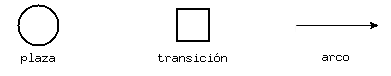
\includegraphics[width=75mm]{Partes_De_Una_Red}
	\caption{Partes de una Red de Petri}
	\label{fig:partes_de_una_red}
\end{figure}

Se pueden visualizar las partes de una Red de Petri en la figura
\ref{fig:partes_de_una_red}.\\


\begin{figure}[h]
    \centering
    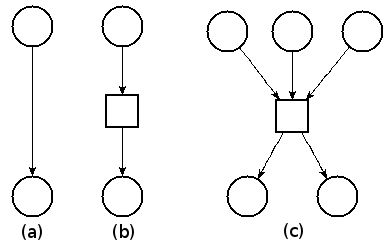
\includegraphics[height=40mm]{Automata_Y_Petri}
    \caption{Equivalencia entre una Máquina de Estados y una Red de Petri}
    \label{fig:automata_y_petri}
\end{figure}

En la figura \ref{fig:automata_y_petri} se aprecia:\\
\begin{itemize}
  \item[(a)] Una máquina de estados de dos estados y una transición.
  \item[(b)] Una RdP equivalente a la máquina de (a).
  \item[(c)] Una RdP con una transición con múltiples arcos de entrada y de
  salida.
\end{itemize}

Se puede extraer como consecuencia directa de esta extensión de la semántica de
un autómata que en una Red de Petri:
\begin{itemize}
  \item Múltiples tokens pueden existir en el modelo al mismo tiempo, y
  particularmente en una plaza.
  \item No existe un estado global explícito.
  \item El estado global del sistema es el conjunto de todos los estados
  parciales, representados por las plazas y sus tokens. A este conjunto se lo
  denomina el \textbf{marcado} de la red.
\end{itemize}

\subsection{Definición Formal de Red de Petri}
\label{def_formal_petri}
A fin de eliminar ambigüedades, se presenta una serie de definiciones sobre
Redes de Petri.

\begin{itemize}
  \stepcounter{definitionsCounter}
  \item [\underline{Definición \thedefinitionsCounter}:] Una Red de Petri R está
  definida por la tupla $(P, T, Pre, Post)$ donde:
  \begin{itemize}
    \item $ P = \{ p_1, p_2, \ldots, p_p \} $ un conjunto de plazas.\footnote{Se
    utiliza $p$ como la cantidad de plazas de la RdP en todo momento dentro de este informe por simplicidad para el lector}
    \item $ T = \{ t_1, t_2, \ldots, t_t \} $ un conjunto de transiciones, donde
    $ P \cap T = \emptyset $. \footnote{Se utiliza $t$ como la cantidad de
    transiciones de la RdP en todo momento dentro de este informe por
    simplicidad para el lector}
    \item $ Pre: P \times T \rightarrow \mathbb{N}^{p} $ aplicación de
    precedencia.\footnote{Se toma la definición de números naturales incluyendo
    el cero por simplicidad de notación.}
    \item $ Post: P \times T \rightarrow \mathbb{N}^{p} $ aplicación de
    incidencia.
  \end{itemize}
  $ Pre (p_i, t_j) $ contiene el peso del arco que va de $ p_i $ a $ t_j $, y
  $ Post (p_i, t_j) $ contiene el peso del arco que va de $ t_j $ a $ p_i $

  \stepcounter{definitionsCounter}
  \item [\underline{Definición \thedefinitionsCounter}:] Una Red de Petri Marcada está
  definida por el par $(R, M)$, donde R es una RdP y $ M : P \rightarrow
  \mathbb{N}^{p}$ (donde $\left\vert{P}\right\vert = p $) es una aplicación
  llamada \textit{marcado}.\\
  $m(R)$, o más simplemente $m$ si la red es conocida, define el marcado de la
  RdP y $m(p_{i})$ o $m_{p_{i}}$ indica el marcado de la plaza $p_{i}$, es
  decir, el número de tokens contenido en la plaza $p_{i}$.\\
  La marca inicial se denota $m_{0}$ y da la cantidad inicial de tokens en todas
  las plazas de la red, por lo que especifica el estado inicial del sistema.
  
  \stepcounter{definitionsCounter}
  \item [\underline{Definición \thedefinitionsCounter}:] Para una marca $m$, una transición $t_{j}$
  está sensibilizada, y por lo tanto es disparable, si y solo si:\\
  $$ \forall p_{i} \in P, m(p_i) \geq Pre(p_{i}, t_{j}) $$
  Conceptualmente, una transición está sensibilizada si todas sus plazas de
  entrada contienen al menos la cantidad de tokens que indica el peso de los
  arcos que las unen.

  En la figura \ref{fig:transiciones_no_sensibilizadas} se observa gráficamente esta definición mediante dos casos de transiciones no sensibilizadas. Nótese
  el peso de los arcos.

  \begin{figure}[h]
    \centering
    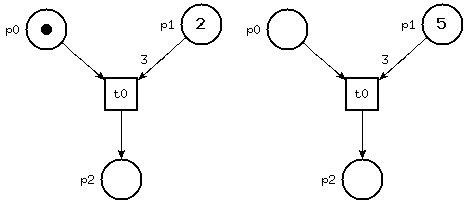
\includegraphics[height=40mm]{Transiciones_No_Sensibilizadas}
    \caption{Ejemplos de transiciones no sensibilizadas.}
    \label{fig:transiciones_no_sensibilizadas}
  \end{figure}
  
  \stepcounter{definitionsCounter}
  \item [\underline{Definición \thedefinitionsCounter}:] La estructura de una Red de Petri
  se denota $ N = \{P, T, F, W\} $ donde,
  \begin{itemize}
    \item $P$ es en conjunto de plazas.
    \item $T$ es el conjunto de transiciones, donde se cumple que $ P \cap T =
    \emptyset $
    \item $F$ es el conjunto de arcos, donde $ F \subseteq (P
    \times T) \cup (F \times P) $.
    \item $W$ es la función de peso de los arcos.
  \end{itemize}

  \stepcounter{definitionsCounter}
  \item [\underline{Definición \thedefinitionsCounter}:] Conjunto de transición y plaza de entrada y
  de salida.
  \begin{itemize}
    \item[] El conjunto de las plazas de entrada a la transición $t$ se denota
    $\bullet t$ y se define,
    $$ \bullet t = \{ p \in P : (p, t) \in F \} $$
    \item[] El conjunto de las plazas de salida de la transición $t$ se denota $
    t \bullet$ y se define,
    $$ t \bullet = \{ p \in P : (t, p) \in F \} $$
    \item[] El conjunto de las transiciones de entrada a la plaza $p$ se
    denota $\bullet p$ y se define,
    $$ \bullet p = \{ t \in T : (t, p) \in F \} $$
    \item[] El conjunto de las transiciones de salida de la plaza $p$ se denota
    $ p \bullet$ y se define,
    $$ p \bullet = \{ t \in T : (p, t) \in F \} $$
  \end{itemize}
\end{itemize}

\subsection{Disparo de una Transición}

La condición de disparo relacionada a $Pre(p_{i}, t_{j})$ significa que para
todas las plazas $p_{i}$ de entrada a $t_{j}$, es decir, todas las plazas que
tienen arcos que apuntan hacia $t_{j}$, el número de tokens presentes debe ser
mayor o igual al peso de dicho arco.

\begin{itemize}
  \stepcounter{definitionsCounter}
  \item [\underline{Definición \thedefinitionsCounter}:] En una RdP, dada una marca $ m_{n}(p) $,
  cualquier transición $ t_{j} $ que se encuentre sensibilizada puede ser
  disparada, y su disparo lleva a una marca $ m_{n+1}(p)$ dada por:
  $$ m_{n+1}(p) = m_{n}(p) + Post(p_{i}, t_{j}) - Pre(p_{i}, t_{j}), \forall
  p_{i} \in P $$
  Como se indica en la ecuación, al disparar la transición $ t_{j} $, se quitan
  tantos tokens de $ \bullet t $ como indiquen los arcos que las unen a $ t_{j}
  $, y se añaden a $ t \bullet $ la cantidad de tokens que indiquen los arcos
  que unen a $ t_{j} $ con ellas.\\
  El disparo de una transición $ t_{j} $ se denota $ m_{n}\rightarrow t_{j}
  \rightarrow m_{n+1} $

  En la figura {\ref{fig:disparo_transicion}} se observa el estado de una RdP
  antes y después del disparo de una transición.
  \begin{figure}[h]
    \centering
    \subfigure[$t_{0}$ sensibilizada]{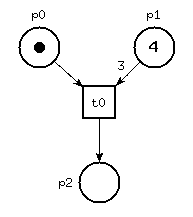
\includegraphics[height=40mm]{Red_Sensibilizada}}
    \subfigure[Disparo de $t_{0}$]{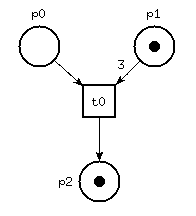
\includegraphics[height=40mm]{Red_Disparada}}
    \caption{Disparo de una transición}
    \label{fig:disparo_transicion}
  \end{figure}
  
  \stepcounter{definitionsCounter}
  \item [\underline{Definición \thedefinitionsCounter}:] Matriz de Incidencia.\\
  La matriz de incidencia de una RdP se define como,
  $$ I = Post - Pre $$
  \textbf{Notas:}
  \begin{itemize}
    \item El disparo de una transición $t_{j}$ se reformula como, $$ m_{n+1}(p)
    = m_{n}(p) + I(p_{i}, t_{j}), \forall p_{i} \in P $$
    \item A partir de las matrices $Pre$ y $Post$ se puede reconstruir la
    estructura de la red, a partir de $I$ no es posible.
  \end{itemize}
\end{itemize}

\subsection{Sucesión de Disparos}

Si en lugar del disparo de una transición se requiere disparar múltiples
transiciones, se puede reescribir la ecuación de cambio de estado de la red de
la siguiente forma,
$$ m_{n+1} = m_{n} + I \times \sigma $$
En esta ecuación, $\sigma$ representa la sucesión de disparos a realizar. Se
cumple $\sigma \in \mathbb{N}^{t}$ y el elemento $\sigma_{i}$ contiene la
cantidad de disparos a realizar sobre $t_{i}$.\\
Si se comienza a realizar la sucesión de disparos $\sigma_{i}$ a partir del
marcado inicial $m_{0}$ y todos los disparos son exitosos, se llega a un marcado
$m_{i}$ y se dice que $m_{i}$ es \textit{alcanzable}.\\
De la misma forma, si existe un marcado $m_{j}$ alcanzable desde $m_{0}$, debe
exitir una sucesión de disparos $\sigma_{j}$ que permita alcanzarlo.

\section{Extensión de la Semántica de las Redes de Petri}

Las RdP descriptas anteriormente constituyen la versión más simple de este
modelo, conocidas como \textit{Redes de Petri Plaza-Transición} o \textit{Redes
de Petri Ordinarias}.

Se pueden realizar modificaciones sobre el modelo a fin de aumentar la semántica
y permitir modelar mayor cantidad de sistemas del mundo real.

Algunas de las variantes introducidas a las RdP desde su aparición son:
\begin{itemize}
  \item Semántica Temporal: Permiten modelar restricciones temporales sobre la
  acciones.
  \item Semántica Estocástica: Permiten modelar restricciones ligadas a 
  variables aleatorias.
  \item Arcos Especiales: Tienen alguna característica que aumenta la
  expresividad de la red.
  \item Tokens Coloreados: Permite asociar un dato (color) a cada token y tomar
  decisiones a partir de su color.
\end{itemize}
\cite{PetriNetsFundamentals}

A continuación se detallan las extensiones que son de interés a este proyecto
integrador.

\subsection{Arcos Especiales}

Durante el modelado de un sistema, en algunas ocasiones es necesario verificar
condiciones más allá de la simple existencia de un recurso esperado.
Cuando esto sucede, una RdP ordinaria no tiene la suficiente expresividad para
modelar esta situación.

Por esto se introducen algunos tipos especiales de arcos que afectan a la
sensibilización de la transición a la que apuntan.

\subsubsection{Arcos Inhibidores}

Un arco inhibidor conecta una plaza $p_{i}$ con una transición $t_{j}$. Si
$m_{p_i} > 0$, entonces $t_{j}$ queda des-sensibilizada.
Este tipo de arcos permite modelar prioridades y ausencia de ciertos recursos.

\subsubsection{Arcos de Reset}

Un arco de reset conecta una plaza $p_{i}$ con una transición $t{j}$,
habilitándola si $m_{p_{i}} > 0$.
Cuando $t_{j}$ es disparada, $m_{p_{i}}$ pasa a valer cero.

\subsubsection{Arcos Lectores}

Un arco lector conecta una plaza $p_{i}$ con una transición $t_{j}$ y tiene un
peso $w$.
$p_{i}$ sensibiliza a $t_{j}$ sólo si $m_{p_{i}} > w$, de la misma manera que
sucede con los arcos estándar, pero el disparo de $t_{j}$ no modifica
$m_{p_{i}}$.

\begin{figure}[h]
  \centering
  \subfigure[Arco Inhibidor]{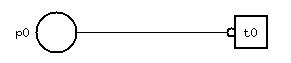
\includegraphics[height=12mm]{Arco_Inhibidor}}
  \subfigure[Arco Lector]{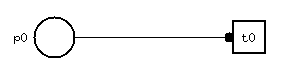
\includegraphics[height=13mm]{Arco_Lector}}
  \subfigure[Arco de Reset]{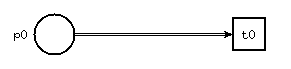
\includegraphics[height=13mm]{Arco_Reset}}
  \caption{Arcos Especiales}
  \label{fig:arcos_especiales}
\end{figure}

\subsection{Guardas}

% QUEREMOS EXTENDER EL MECANISMO DE SENSIBILIZADO
% POR AHORA LA SENSIBILIZACIÓN DEPENDE DEL ESTADO DE LA RED (MARCADO)

% ESTO PERMITE EXTENDER LA SENSIBILIZACIÓN DE FORMA NO AUTÓNOMA, PERMITE ASOCIAR
% LA SENSIBILIZACIÓN A UN ESTADO DEL MEDIO EXTERIOR
% LA GUARDA HACE UN AND CON LA FUNCIÓN DE SENSIBILIZACIÓN PARA DARLE MAYOR FLEXIBILIDAD
% LA GUARDA PUEDE SER POR TRUE O FALSE

Como se describió en la sección \ref{def_formal_petri}, una transición $t_{j}$
se encuentra sensibilizada si $$ \forall p_{i} \in \bullet t_{j}, m(p_i) \geq Pre(p_{i}, t_{j}) $$
Esto es, la sensibilización de $t_{j}$ depende únicamente del estado de
la red para un instante dado.

Si se pretende relacionar la RdP al estado del medio (estado de un sensor, del
programa que se ejecuta, etc), el modelo actual resulta no ser suficientemente
expresivo. Por esta razón, se introduce el concepto de \textit{guarda}.

Sea $V$ un conjunto de \textit{variables booleanas} con $v_{i} \in V$ y tal que
$\left\vert V \right\vert \leq \left\vert T \right\vert$

Si se asocia $v_{i}$ a $t_{j}$, se obtiene la guarda $g_{j}$ que puede tomar el
valor de $v_{i}$ o de su complemento $!v_{i}$ o $\mathtt{\sim} v_{i}$.

Cada variable $v_{i}$ afecta al sensibilizado de todas las transiciones que la
tengan asociada a través de cada guarda $g_{j}$, definiendo una nueva semántica
de sensibilización. Esta se resuelve realizando una operación AND entre el
estado de sensibilización de $t_{j}$ y el estado de su guarda asociada $g_{j}$.

A fin de formalizar este concepto, se construye un vector booleano $SG$ de
dimensión $t = \left\vert{T}\right\vert$, que se obtiene a partir de la
siguiente ecuación:

$$ SG = (V \times RP) \vee ( NV \times RN) \vee (NGT) $$
donde:
\begin{itemize}
  \item $NV \in B^{1 \times \left\vert V \right\vert} \slash  nv_{i} = \neg
  v_{i}$, el vector de variables $v_{i}$ negadas.
  \item $RP \in B^{\left\vert V \right\vert \times \left\vert T 
  \right\vert} \slash rp_{i,j} = True \Leftrightarrow g_{j} \in G \land g_{j} =
  v_{i} $, es decir que $t_{j}$ tiene asociada $g_{j}$ a $v_{i}$.
  \item $RN \in B^{\left\vert V \right\vert \times \left\vert T 
  \right\vert} \slash rp_{i,j} = True \Leftrightarrow g_{j} \in G \land g_{j} =
  \neg v_{i} $, es decir que $t_{j}$ tiene asociada $g_{j}$ a $!v_{i}$.
  \item $NGT \in B^{1 \times \left\vert T \right\vert} \slash ngt_{j} = True
  \Leftrightarrow g_{j} \not \in G$, es decir que $t_{j}$ no tiene guarda
  asociada.
  \item $\vee: B^{1 \times x} \rightarrow B^{1 \times x}$ es la
  función OR elemento a elemento (bitwise).
  \item $\times: B^{n \times m} \times B^{m \times p} \rightarrow B^{n \times
  p}$ es la función multiplicación de matrices booleanas.
\end{itemize}

De esta manera, $sg_{j}$ será $True$ si:
\begin{itemize}
  \item $t_{j}$ no tiene una guarda asociada
  \item El valor de la variable $v_{i}$ coincide con el de la guarda $g_{j}$
  asociada a $v_{i}$
\end{itemize}

Luego, si $f$ es la función de sensibilización utilizada hasta este punto, la
nueva función de sensibilización $f_{ext}$ es:
$$ f_{ext} = f \land SG $$

En la figura \ref{fig:guarda} se observa una plaza unida a una transición,
con una guarda asociada, referida a la variable \textit{\textbf{var}},
habilitada por $True$.

\begin{figure}[h]
  \centering
  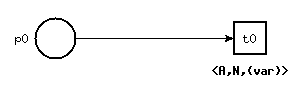
\includegraphics[height=15mm]{Guarda}
  \caption{Transición con guarda}
  \label{fig:guarda}
\end{figure}

\subsection{Semántica Temporal}

Muchos sistemas reales son dependientes del tiempo entre otras variables. Si
resulta de interés modelar un sistema de esta naturaleza, una RdP ordinaria no
es suficiente para hacerlo.

A raíz de esto es que se agrega comportamiento temporal a la semántica del
disparo de las Redes de Petri para obtener \textit{Redes de Petri Temporales}.

Entre las propuestas para agregar semántica temporal a las RdP, son del interés
de este proyecto integrador las Redes de Petri con semántica de \textit{Tiempo
Fuerte} y de \textit{Tiempo Débil}.

\subsubsection{Semántica de Tiempo Fuerte}

En sistemas del mundo real, las actividades no ocurren instantáneamente. Cada
actividad en un sistema tiene una duración distinta de cero, y se deberá asumir
que termina en un tiempo finito para poder modelarla.
\cite{Ramchandani:1974:AAC:889750}

En las RdP con semántica de tiempo fuerte, se asume que el disparo de una
transición toma un tiempo limitado, distinto de cero.

\begin{itemize}
  \stepcounter{definitionsCounter}
  \item [\underline{Definición \thedefinitionsCounter}:] Una Red de Petri Temporal con Semántica de
  Tiempo Fuerte es una tupla $(R, \Omega)$ donde:
  \begin{itemize}
    \item $R$ es una Red de Petri Ordinaria $R = \{P, T, F, W \}$
    \item $\Omega: T \rightarrow \mathbb{R^{+}}$ es una función que asigna
    a cada transición $t_{i} \in T$ un número real no negativo $\tau_{i}$,
    donde $\tau_{i}$ es el \textit{tiempo de disparo de} $t_{i}$
  \end{itemize}
\end{itemize}

\paragraph{Disparo de una Transición con Semántica de Tiempo Fuerte:}

Si $t_{i}$ es una transición que se encuentra sensibilizada, se la puede
disparar. Cuando se inicia el disparo, se retira la cantidad de tokens
correspondiente de $\bullet t_{i}$ y se dice que la transición $t_{i}$
\textit{se está ejecutando}.
La ejecución de $t_{i}$ dura un tiempo $\tau_{i}$, el tiempo de disparo de
$t_{i}$.
Cuando termina de transcurrir el tiempo $\tau_{i}$, se colocan los tokens
correspondientes en $t_{i} \bullet$ y se dice que el disparo \textit{ha
finalizado}.

No se permite comenzar el disparo de una transición que está ejecutando un
disparo anterior, es decir que por transición puede existir un único disparo en
ejecución.

Nótese que el disparo de una transición, pese a haber dejado de ser
instantánteo, sigue siendo atómico como en una RdP ordinaria.

\begin{figure}[h]
  \centering
  \subfigure[Antes]{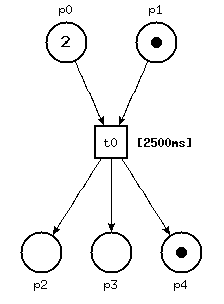
\includegraphics[height=45mm]{Tiempo_Fuerte_01}}
  \subfigure[Ejecución]{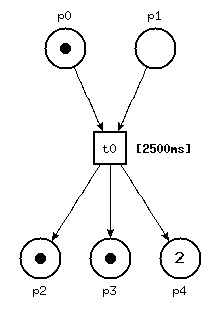
\includegraphics[height=45mm]{Tiempo_Fuerte_02}}
  \subfigure[Terminado]{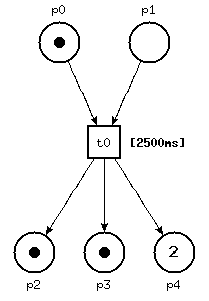
\includegraphics[height=45mm]{Tiempo_Fuerte_03}}
  \caption{Disparo de una transición con semántica de tiempo fuerte}
  \label{fig:disparo_tiempo_fuerte}
\end{figure}

En la figura \ref{fig:disparo_tiempo_fuerte} se observa una transición con
semántica de tiempo fuerte con tiempo de disparo de 2500ms en las tres fases del
disparo.

\subsubsection{Semántica de Tiempo Débil}

De forma más general que la Semántica de Tiempo Fuerte, la Semántica de
Tiempo Débil asigna a una transición $t$ un intervalo $[\alpha, \beta]$
denominado el \textit{intervalo de disparo} de $t$. Este intervalo puede ser cerrado o
abierto en cualquiera de sus extremos, y puede extenderse hasta el infinito. El
disparo de una transición sólo está permitido dentro de su intervalo de disparo.

Los tiempos $\alpha$ y $\beta$ son relativos al último instante de
sensibilización de $t$.
Esto es, si $t$ se sensibilizó por última vez en el instante $\theta$, el
disparo de $t$ sólo será posible en el intervalo $[\theta + \alpha, \theta
+ \beta]$. \cite{PetriNetsFundamentals}

\begin{itemize}
  \stepcounter{definitionsCounter}
  \item [\underline{Definición \thedefinitionsCounter}:] Una Red de Petri Temporal con Semántica de
  Tiempo Débil es una tupla $(R, IS)$ donde:
  \begin{itemize}
    \item $R$ es una Red de Petri Ordinaria $R = \{P, T, F, W \}$
    \item $IS: T \rightarrow \mathbb{Q^{+}} \times \{ \mathbb{Q^{+}} \cup \{
    \infty \} \}$ es la función de \textit{intervalo estático}.
  \end{itemize}
\end{itemize}

La función $IS$ asigna a cualquier transición $t \in T$ un intervalo con límites
racionales $IS(t) = [\alpha, \beta]$, con $0 \leq \alpha \leq \beta$. Solamente
$\beta$ puede adquirir un valor infinito.

El disparo de $t$ sólo está permitido en el intervalo de tiempo que tenga
relacionado. En el instante inicial (tiempo = 0), si $t$ está sensibilizada por
el marcado inicial, este intervalo coincide con el intervalo estático $IS(t)$.
Cuando el tiempo transcurre, el intervalo de $t$ avanza, corriéndose hacia el
origen una cantidad de tiempo igual al transcurrido desde el instante de
sensibilización. A este intervalo se le llama \textit{intervalo dinámico de disparo.}

Estos intervalos dinámicos pueden ser expresados como una aplicación $I$ que
asigna a cada transición $t$, un intervalo de tiempo $I(t)$ en el cual puede ser
disparada. Los límites del intervalo $I(t)$ son denominados el \textit{instante
menor de disparo} y el \textit{instante mayor de disparo}
correspondientemente. y son denotados $DMin(t)$ y
$DMax(t)$.\cite{PetriNetsFundamentals}

\paragraph{Estado de una Red de Petri Temporal:}

El estado de una RdP con Semántica de Tiempo Débil es un par $E = (M, I)$ donde
$M$ es el marcado de la red e $I$ es la \textit{aplicación de intervalos de
disparo}. El estado inicial $E_{0}$ consiste en la marca inicial $M_{0}$ y la
aplicación $I_{0}$ que asigna a cada transición sensibilizada su intervalo
estático y a las transiciones no sensibilizadas, el intervalo vacío.
Disparar una transición $t_{i}$ en el instante $\theta$ está permitido desde un
estado $E$, únicamente si se cumple:
\begin{itemize}
  \item La transición $t_{i}$ está sensibilizada por el marcado M.
  \item $\theta$ no es menor que el instante menor de disparo de $t_{i}$
  $$\theta \geq DMin(t_{i})$$
  \item $\theta$ no es mayor que el instante mayor de disparo de cualquier
  transición habilitada por $M$
  $$ \forall k, M \geq Pre(k) \Rightarrow \theta \leq DMax(k) $$
\end{itemize}

\paragraph{Disparo de una transición con Semántica de Tiempo Débil:}

El disparo de una transición $t_{i}$ en el instante $\theta$, desde el estado
$E = (M,I)$ lleva al estado $E' = (M', I')$ determinado de la siguiente manera:
\begin{itemize}
  \item El marcado $M'$ se determina igual que en una RdP Ordinaria.
  \item El intervalo $I'(t_{j})$ para cada transición $t_{j}$ se define:
  $$ I'(t_{i}) = \left\{
  \begin{array}{lll}
    \textnormal{Intervalo vacío} & si & t_{j} \textnormal{ no esta sensibilizada
    por } M \\
    IS(t_{j}) & si & t_{j} \textnormal{ entra en conflicto con } t_{i} \\
    \lbrack max(0, DMin(t_{j}) - \theta), DMax(t_{j}) - \theta \rbrack & si &
    t_{j} \textnormal{ está sensibilizada y } DMax(t_{j}) \in \mathbb{Q} \\
    \lbrack max(0, DMin(t_{j}) - \theta), \infty \rbrack & si & t_{j}
    \textnormal{ está sensibilizada y } DMax(t_{j}) = \infty \\
  \end{array}
\right.$$
\end{itemize}
Nótese que, a diferencia de la semántica de tiempo fuerte, el disparo de $t_{i}$
es instantáneo.

\begin{figure}[h]
  \centering
  \subfigure[Antes]{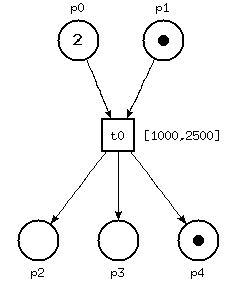
\includegraphics[height=45mm]{Tiempo_Debil_01}}
  \subfigure[Después]{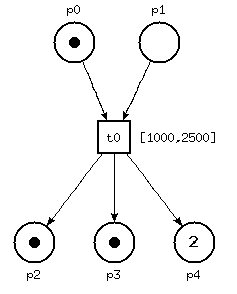
\includegraphics[height=45mm]{Tiempo_Debil_02}}
  \caption{Disparo de una transición con semántica de tiempo débil}
  \label{fig:disparo_tiempo_debil}
\end{figure}

En la figura \ref{fig:disparo_tiempo_debil} se observa el instante anterior y
posterior al disparo de una transición con semántica de tiempo débil. Para que
esto ocurra, el instante de disparo tiene que encontrarse dentro del intervalo
dinámico de disparo de $t_{0}$.

\begin{figure}[h]
  \centering
  \hspace*{\fill}
  \subcapcentertrue
  \subfigure[Transición con semántica de tiempo fuerte] {
    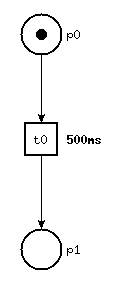
\includegraphics[align=c,height=50mm]{Tiempo_Fuerte_04}
    \label{fig:tiempo_debil_emula_fuerte_Fuerte}
  }
  \subfigure[Transición con semántica de tiempo fuerte modelada por transiciones
  con semántica de tiempo débil] {
    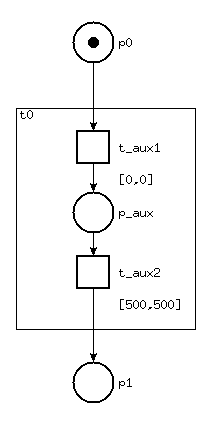
\includegraphics[align=c,height=75mm]{Tiempo_Debil_Emula_Fuerte}
    \label{fig:tiempo_debil_emula_fuerte_Debil}
  }
  \hspace*{\fill}
  \caption{Transición de tiempo fuerte modelada por tiempo débil}
  \label{fig:tiempo_debil_emula_fuerte}
\end{figure}

En la figura \ref{fig:tiempo_debil_emula_fuerte} se observa cómo, utilizando
transiciones temporales de semántica de tiempo débil, se puede modelar el
comportamiento de una transición de semántica de tiempo fuerte.
Para entender esta equivalencia, es conveniente repasar mediante un ejemplo el
disparo en ambos casos.

\subparagraph{Disparo en Tiempo Fuerte:}
Como se observa en la figura \ref{fig:tiempo_debil_emula_fuerte_Fuerte}, $t_{0}$ se
encuentra sensibilizada.
\begin{itemize}
  \item En el instante $\tau = 0$ se dispara $t_{0}$.
  \item Automáticamente se retira un token de $p_{0}$.
  \item Durante 500 milisegundos no ocurre nada.
  \item En $\tau = 500ms$ se coloca un token en $p_{1}$.
\end{itemize}

\subparagraph{Disparo en Tiempo Débil:}
Nuevamente, en la figura \ref{fig:tiempo_debil_emula_fuerte_Debil}, $t_{0}$ se
encuentra sensibilizada.
\begin{itemize}
  \item En el instante $\tau = 0$ se dispara $t_{aux1}$. Esto es posible ya que
  el intervalo de tiempo asociado lo permite.
  \item Se retira un token de $p_{0}$ y se coloca otro en $p_{aux}$.
  \item En ese instante se sensibiliza $t_{aux2}$ y se establece su intervalo dinámico.
  \item Durante 500 milisegundos no se puede disparar $t_{aux2}$.
  \item En $\tau = 500ms$ se dispara $t_{aux2}$, colocándo un token en $p_{1}$.
\end{itemize}

Así, visto desde el punto de vista de $p_{0}$ y $p_{1}$, en ambos casos el
comportamiento fue idéntico, con lo que se puede afirmar que la
semántica de tiempo débil tiene mayor expresividad y por lo tanto, es capaz de
modelar más situaciones del mundo real que la semántica de tiempo fuerte.


\subsection{Autonomía de una RdP}

Las redes de Petri analizadas en las secciones anteriores permiten modelar el
comportamiento de sistemas describiendo \textbf{qué} sucede en un proceso pero
no \textbf{cuándo} sucede.

Comunicando la RdP con el exterior del modelo, se puede controlar el momento (o
al menos el orden) con el que suceden los eventos. De esta manera, la RdP pasa a
ser \textit{no autónoma}.

\subsubsection{Red de Petri Autónoma}

En una RdP autónoma, se sabe que una transición puede ser disparada si está
sensibilizada, pero no se sabe cuándo o por qué será disparada.

Una extensión sobre este modelo son las \textit{\textbf{Redes de Petri
Estocásticas}}, donde a cada transición se le asigna una variable aleatoria
booleana $X$ con función de distribución de probabilidades $f$, que determina la
probabilidad de que se realice un disparo en un instante dado, si la marca $M$ lo permite.

Este tipo de modelos resulta súmamente útil para simular el comportamiento de
muchos sistemas del mundo real, ligados a variables aleatorias.

\subsubsection{Red de Petri No Autónoma}
En una RdP no autónoma, se asocia un evento $E^{i}$ a cada transición $t_{j}$ y
el disparo se da si $t_{j}$ está sensibilizada y $E^{i}$ ocurre.

Los \textit{eventos externos} corresponden a un cambio en el estado del medio
(incluyendo el tiempo). En cambio, un cambio del estado interno (del marcado),
se denomina \textit{evento interno}. La ocurrencia de un evento no tiene
duración. \cite{Hybrid_petri_nets}

\begin{itemize}
  \stepcounter{definitionsCounter}
  \item [\underline{Definición \thedefinitionsCounter}:] Una RdP sincronizada es una tupla
  $RdP_{Sync} = \{R, E, Sync\}$ tal que:
  \begin{itemize}
    \item $R =  \{P,T,F,W\}$ es una Red de Petri marcada.
    \item $E$ es un conjunto de eventos externos.
    \item $Sync : T \rightarrow (E \cup \{e\} ) $ donde $e$ es el evento
    que ocurre siempre.
  \end{itemize}
  \stepcounter{definitionsCounter}
  \item [\underline{Definición \thedefinitionsCounter}:] En una RdP no autónoma, una transición $t$
   es \textit{inmediata} o \textit{automática} si es disparada $q$ veces cuando
   está \textit{q-sensibilizada} $\forall q > 0$, a menos que existan conflictos
   entre dos o más transiciones.
\end{itemize}

Se dice que una transición sujeta a un evento externo es \textit{disparada}, de
otro modo será \textit{automática}. Esto se identifica en el modelo con una
etiqueta \textit{D} o \textit{F} para una transición disparada, y \textit{A}
para una automática.

\paragraph{Eventos estocásticos en redes de Petri no autónomas:}
Si una transición $t_{j}$ está sensibilizada, es disparada y espera la
ocurrencia del evento $E^{n}$ se disparará cuando $E^{n}$ ocurra.
Si a su vez se construye un generador de eventos $E^{n}$ sujeto a una variable
aleatoria $X$ con distribución de probabilidad $f$, se puede replicar la
semántica de una RdP estocástica utilizando una RdP no autónoma.
\footnote{Esta técnica se puede utilizar para depurar el modelo, agregando
eventos mediante simulación}

\subsection{Informes de Disparo}

De la misma forma que una RdP no autónoma permite actuar en función de eventos
provenientes del mundo exterior, los informes de disparo le brindan a la RdP la
posibilidad de emitir eventos hacia el medio. A su vez, estos eventos pueden
desencadenar acciones en observadores del mundo externo.

Una transición que emite eventos se denomina \textit{informada}.
Esto se denota con una etiqueta en la transición, indicando \textit{I} si es
informada, o \textit{N} si no lo es.

Para demostrar el potencial de este mecanismo, se analiza el siguiente ejemplo:

\begin{figure}[h]
  \centering
  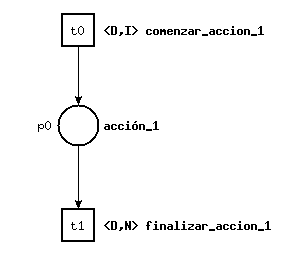
\includegraphics[height=50mm]{Emitir_Eventos_01}
  \caption{Emisión de Eventos ligados a acciones}
  \label{fig:eventos01}
\end{figure}

Si se relaciona una plaza $p_{0}$ con la ejecución de una
\textit{acción\textunderscore1} en el modelo, se puede aprovechar el mecanismo
de informes para sincronizar esta acción.

A continuación se describe una sucesión de eventos que aprovecha este
mecanismo, referido a la RdP de la figura \ref{fig:eventos01}:
\begin{itemize}
  \item Sucede un evento $E_{ext}^{0}$, $t_{0}$ lo escucha y de dispara.
  \item $t_{0}$ emite un evento $E_{int}^{0}$ avisando que fue disparada.
  \item Un observer de $E_{int}^{0}$ ejecuta \textit{acción\textunderscore1}.
  \item La finalización de \textit{acción\textunderscore1} emite un evento
  $E_{ext}^{1}$ hacia la RdP.
  \item $t_{1}$ escucha el evento $E_{ext}^{1}$ y se dispara.
\end{itemize}

\subsection{Política de Selección de Disparo}

Si existen múltiples transiciones sensibilizadas en una RdP, resulta de interés
tener un mecanismo de decisión que indique cuál debería ser la próxima
transición disparada.
Esta decisión resulta particularmente significativa en el caso de que dos o más
transiciones se encuentren en conflicto, ya sea un conflicto inmediato o un
conflicto que se genere luego de aplicar una sucesión de disparo $\sigma$.

El análisis del surgimiento de conflictos y de su posible resolución en redes de
Petri, lleva a algoritmos de búsqueda en árboles, con lo que su complejidad
crece exponencialmente con la profundidad del árbol a analizar, es decir, con
la cantidad de disparos futuros a analizar y con la cantidad de transiciones
analizadas. Esto lo hace imposible de aplicar para resolver problemas de
decisión de disparo por medio de la heurística.

La \textit{Política de Selección de Disparo} se refiere a la elección de la
próxima transición a disparar entre todas las sensibilizadas. Para una RdP,
incluidas la no autónomas o temporales, si esta elección es aleatoria el sistema
resulta no determinístico. Para que el sistema sea determinístico hay diferentes
soluciones, como la inclusión de: prioridades, probabilidades, arcos
inhibidores, arcos lectores. etc. \cite{Ecuacion_generalizada_LAC}

La política de selección de disparo $P : TS \rightarrow t \slash TS \subseteq T
\land t \in TS $ es una función que dado un vector de transiciones
sensibilizadas $TS$ indica cuál transición $t$ deberá ser disparada.

Para un determinado problema a resolver con una RdP, con conocimiento del
dominio del problema se puede diseñar una política de selección de disparos que
contemple los conflictos que puedan surgir, y priorice el disparo de
transiciones que generen situaciones más favorables para la solución de dicho
problema.

Cabe destacar que, pese a obtener un diseño correcto del modelo, una política
desfavorable al problema a tratar puede beneficiar ampliamente a parte de la
ejecución del modelo y perjudicar a otras, generando inanición sobre estas.


\section{Comparación entre Redes de Petri y Autómatas}

Comparado a los autómatas, las RdP ofrecen una representación compacta de
sistemas concurrentes. Por esto, el modelado de este tipo de sistemas es
usualmente más natural usando redes de Petri. \cite{Iordache:2006:SCC:1197724}

Para comparar RdP y autómatas, se consideran sistemas compuestos por varios
subsistemas y se compara el tamaño de la RdP y el autómata que modelan el
sistema completo.

A fin de realizar esta comparación, es necesario previamente definir la
composición de autómatas y de redes de Petri.\cite{Iordache:2006:SCC:1197724}

\begin{itemize}
  \stepcounter{definitionsCounter}
  \item [\underline{Definición \thedefinitionsCounter}:] Sean $G_{1} = (Q_{1}, \Sigma_{1},
  \delta_{1}, s_{1}, F_{1})$ y $G_{2} = (Q_{2}, \Sigma_{2}, \delta_{2}, s_{2},
  F_{2})$ autómatas no determinísticos. La \textit{Composición Paralela} o
  \textit{Síncrona} de $G_{1}$ y $G_{2}$ es un autómata $G = G_{1} \parallel
  G_{2}$ que se define:
  $$ G = Ac(Q_{1} \times Q_{2}, \Sigma_{1} \cup \Sigma_{2}, \delta, (s_{1},
  s_{2}), F_{1} \times F_{2}) $$ donde $Ac$ es la función que elimina los estados no
 alcanzables de un autómata y $ \delta $ se define de la siguiente forma:
 \begin{itemize}
  \item [\underline{Definición \thedefinitionsCounter.1}:] Sea
   $$ \bar{\delta_{i}}(q,\alpha) =
   \left\{ 
     \begin{array}{lll}
      \delta_{i}(q, \alpha) & & \forall \alpha \in \Sigma_{i} \\
      \{q\} & & \forall \alpha \in (\Sigma_{1} \cup \Sigma_{2} \cup \{\lambda\})
      \backslash \Sigma_{i}
     \end{array}
   \right. $$
   para $i = 1,2$ y donde $\lambda$ es el evento nulo y $\backslash$ es la
   operación resta de conjuntos.
   Entonces: $$ \delta((q_{1},
   q_{2}), \alpha) = \bar{\delta_{1}}(q_{1}, \alpha) \times \bar{\delta_{2}}(q_{2}, \alpha) $$
 \end{itemize}
\end{itemize}

A fin simplificar el entendimiento de la composición de autómatas, se presenta
el siguiente ejemplo:

\begin{figure}[h]
  \centering
  \subfigure[$G_{1}$]{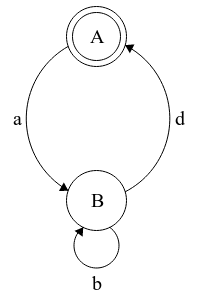
\includegraphics[height=45mm]{Composicion_Automata_1}}
  \subfigure[$G_{2}$]{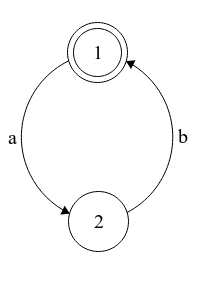
\includegraphics[height=45mm]{Composicion_Automata_2}}
  \subfigure[$G_{1} \parallel G_{2}$]{
    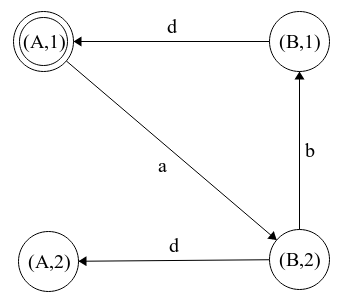
\includegraphics[height=45mm]{Composicion_Automata_3}
  }
  \caption{Composición de Autómatas}
  \label{fig:composicion_automatas}
\end{figure}

Sean $$G_{1} = (\{A, B\}, \{a, b, d\}, \delta_{1}, A, \{B\})$$ y $$G_{2} = (\{1,
2\}, \{a, b\}, \delta_{2}, 1, \{2\})$$ dos autómatas, entonces $G = G_{1}
\parallel G_{2}$ tendrá:
\begin{itemize}
  \item Estado inicial $(A, 1)$ ya que $A$ y $1$ son ambos estados iniciales.
  \item Estados finales $\{(B, 2)\}$ ya que $B$ y $2$ son estados finales.
  \item Las transiciones son:
  \begin{itemize}
    \item De $(A,1)$ a $(B,2)$ etiquetada con $a$ porque hay una transición de
    $A$ a $B$ y otra de $1$ a $2$, ambas etiquetadas con $a$.
    \item De $(B,2)$ a $(B,1)$ etiquetada con $b$ porque hay una transición de
    $B$ a $B$ y otra de $1$ a $2$, ambas etiquetadas con $b$.
    \item De $(B,1)$ a $(A,1)$ etiqueada con $d$, porque en $G_{1}$ hay una
    transición de $B$ a $A$ etiquetada con $d$, y como $d$ no existe en el
    conjunto de símbolos de $G_{2}$ no puede generar restricciones y según la
    definición genera una transición de $1$ hacia $1$.
    \item De $(B,2)$ a $(A,2)$ etiquetada con $d$ por la misma razón que la
    transición anterior. La transición de $A$ a $B$ existe en $G_{1}$, y se
    genera una de $2$ a $2$ en $G_{2}$
  \end{itemize}
\end{itemize}
    
\paragraph{Tamaño del autómata compuesto:}
Analizando el tamaño del modelo compuesto, asumiendo que todos los estados de
$Q_{1} \times Q_{2}$ son alcanzables desde el estado inicial, si $G_{1}$ tiene
$m_{1}$ estados y $G_{2}$ tiene $m_{2}$ estados, entonces $G_{1} \parallel
G_{2}$ tiene $m_{1} m_{2}$ estados. Es decir que la cantidad de estados de la
composición de autómatas es (o está acotada por) el \textbf{producto} de la
cantidad de estados de los autómatas que lo componen.

\begin{itemize}
  \stepcounter{definitionsCounter}
  \item [\underline{Definición \thedefinitionsCounter}:] Sean $R_{1} = (P_{1}, T_{1}, Pre_{1},
  Pos_{1}, \rho_{1})$ y $R_{2} = (P_{2}, T_{2}, Pre_{2}, Pos_{2}, \rho_{2})$
  redes de Petri etiquetadas donde:
  \begin{itemize}
    \item $\rho_{i} : T_{i} \rightarrow \Sigma_{i} \cup \{ \lambda \}$ para $i =
    1, 2$ es la función de etiquetado de las transiciones de $R_{i}$.
    \item $ \Sigma_{i} $ es el conjunto de símbolos del autómata equivalente a
    la i-ésima red de Petri
    \item $\lambda$ es el evento nulo
  \end{itemize} 
  La composición resulta en una red $R = (P, T, Pre, Pos, \rho)$ tal que $T$
  contiene las transiciones de $T_{1}$ y de $T_{2}$ que no están etiquetadas con
  $\lambda$ y las transiciones $t$ que modelan sincronizaciones de pares
  $(t^{1}, t^{2}) \in T_{1} \times T_{2}$ que comparten etiquetas distintas de
  $\lambda$.
  Se puede construir la red compuesta utilizando el siguiente algoritmo:
  \begin{enumerate}
    \item Sea $P = P_{1} \cup P_{2} $ y $T = \emptyset$.
    \item Sean $L_{1} = \bigcup_{t \in T_{1}} \rho_{2}(t) \backslash
    \{\lambda\}$ y $L_{2} = \bigcup_{t \in T_{2}} \rho_{1}(t) \backslash
    \{\lambda\}$.
    \item Para $i = 1, 2$, sea $T_{i,-} = \{ t \in T_{i}: \rho_{i} \backslash
    L_{i} \not = \emptyset \}$.
    \item Para $i = 1, 2, \forall t \in T_{i,-}$, sea $T = \{t\} \cup T$.
    $\rho(t) = \rho_{i}(t) \backslash L_{i}$. Sea $Pre(p, t) = Pre_{i}(p, t)$ y $Pos(p,
    t) = Post_{i}(p, t) \forall p \in P$ y sea $ Pre(p, t) = 0 $ y $ Pos(p,t) =
    0$ $\forall p \in P \backslash P_{i}$.
    \item Para cada par de transiciones $(t^{1}, t^{2}) \in T_{1} \times T_{2}$
    tal que $(\rho_{1}(t^{1}) \cap \rho_{2}(t^{2})) \backslash \{\lambda\} \not
    = \emptyset$, crear una nueva transición $t : T = {t} \cup T$, $\rho(t) =
    (\rho_{1}(t^{1}) \cap \rho_{2}(t^{2})) \backslash \{\lambda\}$ y hacer
    $Pre(p, t) = Pre_{i}(p,t)$ y $Pos(p, t) = Pos_{i}(p,t)$ $\forall p \in
    P_{i}$ para $i = 1, 2$.
  \end{enumerate}
\end{itemize}

Retomando el ejemplo de la composición de autómatas de la figura
\ref{fig:composicion_automatas}, se presenta la composición de las redes de
Petri equivalentes a dichos autómatas.

\begin{figure}[h]
  \centering
  \subfigure[$R_{1}$]{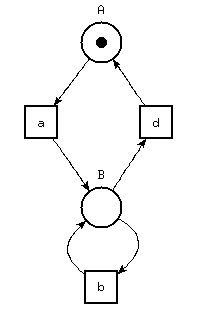
\includegraphics[width=35mm]{Composicion_Petri_1}}
  \subfigure[$R_{2}$]{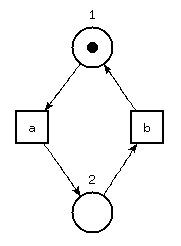
\includegraphics[width=30mm]{Composicion_Petri_2}}
  \subfigure[$R_{1} \parallel R_{2}$]{
    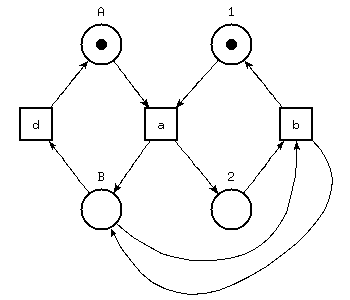
\includegraphics[width=65mm]{Composicion_Petri_3}
  }
  \caption{Composición de Redes de Petri}
  \label{fig:composicion_petri}
\end{figure}

\paragraph{Tamaño de la RdP compuesta:}
Si $R_{1}$ tiene $m_{1}$ plazas y $R_{2}$ tiene $m_{2}$ plazas, entonces $R =
R_{1} \parallel R_{2}$ tendrá $m_{1} + m_{2}$ plazas.
En contraste con el caso del autómata, la red de Petri compuesta crece
linealmente en cantidad de plazas respecto de las redes originales, es decir que
crece con la \textbf{suma} de las plazas de las redes originales.
Además, las transiciones de la red compuesta son las de las redes originales,
unificando las que comparten etiqueta. Es decir que la cantidad de transiciones
del modelo compuesto está acotada por la \textbf{suma} de las cantidades de los
modelos que lo componen.

\paragraph{Conclusión sobre la comparación de modelos:}
Analizando la forma en que crece el modelo resultado de	 la composición de
autómatas contra la composición de RdP se ve que estas últimás son más aptas para el modelado de
manera compacta de sistemas paralelos formados por subsistemas menores.
De la misma manera, una RdP permite modelar sistemas paralelos mucho mayores que
un autómata sin que el modelo resulte demasiado complejo para su análisis.
Otro punto a destacar es la existencia de un algoritmo para la composición de
redes de Petri, lo que permite la automatización de este proceso, simplificando
la tarea de construcción del modelo.

        \chapter{Paradigmas de Programación}
            \section{Paradigma Dataflow}

El paradigma de programación \textit{Dataflow} se basa en la idea de evitar que
el programador piense en términos del flujo de control del programa y se centre
en el flujo de los datos que son procesados.
De esta manera, las aplicaciones son representadas como un conjunto de nodos (o
bloques) con puertos de entrada y/o salida. Estos nodos pueden ser productores,
consumidores o bloques de procesamiento de información que fluye por el sistema. Los nodos
están conectados por aristas que definen el flujo de información por el
sistema. La mayoría de los lenguajes de programación visuales que usan una
arquitectura basada en bloques están basados en el paradigma dataflow.
\cite{DataflowTiagoSousa}

Los nodos son ejecutados únicamente cuando reciben y/o envían mensajes, lo que
sucede asíncronamente respecto de los demás nodos. Por esto, las aplicaciones
dataflow son inherentemente paralelas.\cite{DataflowRichardHarter}

La programación dataflow es capaz de proveer paralelismo sin la complejidad de
la gestión de hilos. Esto es posible gracias a que cada nodo es un bloque de
procesamiento independiente de los demás y no produce efectos colaterales
\cite{DataflowTiagoSousa}

Hay una amplia variedad de lenguajes dataflow, variando de hojas de cálculo,
Labview, hasta Erlang. Muchos son gráficos. La programación se hace alterando
diagramas de flujo. Una característica que tienen todos en común es que tienen
un sistema de ejecución (runtime system).\cite{DataflowRichardHarter}

Los programas imperativos tradicionales están compuestos de rutinas que se
llaman entre sí, por ejemplo, cuando una llamada hace que el llamador construya
un paquete de datos (secuencia de llamada) y transfiere el control y el paquete
de datos a la rutina llamada. Cuando la rutina llamada termina, contruye un
paquete de datos para pasar de vuelta al llamador y le transfiere nuevamente el control.

En los programas dataflow las “rutinas” no se llaman entre sí, en su lugar son
activadas por el sistema de ejecución cuando hay entrada para ellos. Cuando se
crean salidas, el sistema de ejecución se hace cargo de mover la salida al
destino que requiere esas salidas. Cuando las “rutinas” terminan, transfieren el
control de vuelta al sistema de ejecución.

Una diferencia entre la programación imperativa y dataflow es
la semántica utilizada. Mientras la programación imperativa utiliza semántica
LIFO, la dataflow usa semántica FIFO \cite{DataflowRichardHarter}. Eso es, un
programa imperativo pone datos en una pila y obtiene datos desde la misma pila.
En cambio en programas dataflow, cada elemento obtiene datos de una cola y pone
datos en otras colas.
Otra diferencia es que la conectividad de los programas procedurales está
embebida en el código. Para pasar datos de la rutina $A$ a $B$, $A$ debe
llamar explícitamente a $B$, es decir que un llamado tiene que especificar el
destino de los datos.
Por otro lado, en programas dataflow la conectividad puede estar separada
del código, $A$ no pasa datos directamente a $B$; en su lugar, le pasa datos al
sistema de ejecución, quien le pasa los datos a $B$.
El llamador no tiene que especificar hacia dónde van los datos y hasta puede
no saberlo. \cite{DataflowRichardHarter}

\subsection*{Ventajas y Desventajas del paradigma Dataflow}

Entre las ventajas de utilizar el paradigma dataflow se encuentran:

\begin{itemize}
  \item La concurrencia y paralelismo son naturales. El código se puede distribuir entre cores y a través de redes. Algunos
  problemas relacionados a hilos desaparecen
  \item Las redes dataflow son representaciones naturales e intuitivas para
  representar procesos.
  \item El paso de mensajes permite deshacerse de problemas asociados a memoria compartida y locks.
  \item Los programas dataflow son más extensibles que programas tradicionales.
  Los elementos pueden ser agrupados en elementos compuestos.
\end{itemize}

Por otro lado, resulta poco ventajoso utilizar este paradigma por los siguientes
motivos:

\begin{itemize}
  \item El modelo de pensamiento de programación dataflow es poco familiar para
  la mayoría de los programadores profesionales.
  \item La mayoría de los lenguajes de programación dataflow son lenguajes de
  un nicho usado por programadores no profesionales.
  \item La intervención del sistema de ejecución puede tener aparejado un alto
  costo computacional. La gran ventaja de la semántica LIFO es que se implementa
  en código de manera inmediata y poco costosa.
  \item No utilizar memoria compartida tiene sus costos. Los mensajes deben ser
  copiados o deben ser inmutables.
  \item Usar programación dataflow requiere que sea utilizada del principio. De
  esta manera, convertir programas tradicionales en programas dataflow es
  difícil porque la estructura es diferente.
\end{itemize}

\section{Paradigma Reactivo}

El paradigma reactivo es un paradigma de programación construído en torno a
flujos de datos, y la propagación de los cambios sobre ellos. Esto significa que
los lenguajes que implementan este paradigma deben permitir expresar flujos de
datos de manera estática o dinámica con facilidad, y el modelo de ejecución
debe propagar automáticamente los cambios en los datos cuando ocurran,
actualizando todos los valores correspondientes de manera transparente para el
programador.

A fin de comprender las características principales de este paradigma se
presenta el siguiente ejemplo:

\begin{figure}[h!]
\centering
\begin{minted}{perl}
a = 1
b = 2
c = a + b
a = 3
\end{minted}
\end{figure}

En programación imperativa, terminada la ejecución de esta sección de código,
$c$ vale $3$ y así se mantendrá indefinidamente o hasta que el programador le
asigne un nuevo valor. En cambio en programación reactiva el valor de $c$ se
mantiene siempre actualizado, es decir, la expresión declarada como $c$
se vuelve a computar automáticamente ante un cambio en $a$ o en $b$, y en este
ejemplo pasa a valer $5$. Se dice que $c$ es \textit{dependiente} de $a$ y $b$.
\cite{Bainomugisha:2013:SRP:2501654.2501666}

Al igual que en el paradigma dataflow, en el paradigma reactivo son los datos
los que fluyen por el programa en lugar del control. La diferencia radica en
que, bajo el paradigma reactivo, las ``conexiones'' de datos pueden ser
alteradas dinámicamente en tiempo de ejecución.
Además se introducen restricciones de tiempo real blando, para lo cual se
definen dos conceptos:
\begin{itemize}
  \item \textit{Behaviours (Comportamientos)} representan eventos de variación
  contínua en el tiempo. El beahaviour por excelencia es el tiempo, de hecho los
  lenguajes reactivos ofrecen primitivas para representar al tiempo.
  \item \textit{Events (Eventos)} representan eventos discretos. Suelen estar
  representados en forma de flujos de cambios de valores. A diferencia de los
  behaviours, los eventos cambian en instantes puntuales del tiempo. Los
  lenguajes reactivos ofrecen primitivas para combinar y procesar eventos.
\end{itemize}
\cite{Bainomugisha:2013:SRP:2501654.2501666}

\subsection*{El Paradigma Reactivo y El Patrón Observer}

El patrón de diseño \textit{observer} \cite{Gamma:1995:DPE:186897} nace de la
necesidad de mantener consistencia de datos en sistemas particionados, sin generar
acoplamiento entre capas de dichos sistemas.
Permite que un \textit{sujeto} publique cambios en su estado a sus
\textit{observadores}, quienes se susbribieron previamente a estas
actualizaciones.

El patrón observer se debe utilizar en alguna de las siguientes situaciones:
\begin{itemize}
  \item Cuando una abstracción tiene dos partes, una dependiente de la otra.
  \item Cuando el cambio en un objeto implica el cambio en otros, y no se sabe
  de antemano cuántos ni quiénes deben aplicar estos cambios.
  \item Cuando un objeto debe notificar a otros sin conocer nada de ellos, es
  decir sin generar acomplamiento.
\end{itemize}
\cite{Gamma:1995:DPE:186897}

Analizando este patrón de diseño se encuentran similitudes con el paradigma
reactivo.
La programación reactiva es capaz de explicitar mayor granularidad, pudiendo
describir flujos de datos a nivel de clases, miembros de éstas y hasta
variables, mientras que el patrón observer lo puede hacer a nivel de clases
únicamente.

En programación reactiva, cuando se forma una expresión dependiente de otras, se
genera una suscripción implícita de manera automática y el modelo de ejecución
es el encargado de propagar los cambios de manera transparente para el
programador.


            \section{Programación Orientada a Aspectos}
\label{sec:aop}

\subsection{Concepto}

La programación orientada a aspectos es un paradigma de programación que tiene
como objetivo incrementar la modularidad mediante la separación de intereses
transversales (cross-cutting concerns). 
Los intereses transversales son aspectos de un programa que afectan a otros
intereses. Son partes de un programa que afectan o dependen de muchas
otras partes del sistema.
Estos intereses usualmente no pueden separarse claramente del resto del
sistema, y pueden resultar en duplicación de código o un alto grado de
dependencia entre partes del sistema.


Los intereses transversales son la base para el desarrollo de aspectos. Estos no
pueden ser representados claramente en los paradigmas de programación orientado
a objetos o programación procedural.
La separación de intereses transversales se realiza añadiendo comportamientos
adicionales al codigo existente (llamados consejos o advices) sin cambiar el
código existente. En cambio especifica separadamente que codigo debe modificarse
mediante la definición de pointcuts. 

La programación orientada a aspectos complementa a la programación orientada a
objetos al permitir al desarrollador modificar dinamicamente el modelo estático
orientado a objetos para crear un sistema que puede crecer para cumplir nuevos
requerimientos. Tal como los objetos en el mundo real pueden cambiar sus estados
a lo largo de su vida, una aplicación puede adoptar nuevas características a
medida que se va desarrollando. \cite{Introduction_To_Aspect}


\subsection{Terminología}
\label{sec:aop_terminologia}
\begin{itemize}
  \item Intereses Transversales (Cross-cutting concerns): Aunque la mayoría de
  las clases en un modelo orientado a objetos está destinada a perfeccionar una función única y
  específica, usualmente comparten requerimientos secundarios en común con otras
  clases. Por ejemplo, se puede desear añadir mecanismos de logueo a las clases
  dentro de la capa de acceso de datos y también a las clases en la capa de
  interfaz de usuario cada vez que un hilo entre o salga de un método. Aunque la
  funcionalidad principal de cada clase es muy diferente, el código necesario
  para realizar la tarea secundaria es usualmente
  idéntico.\cite{Introduction_To_Aspect}
  
  \item Consejos (Advices): Es el código adicional que se desea aplicar al
  modelo existente. Siguiendo con el ejemplo anterior, es el código de logueo
  que se quiere aplicar cada vez que un hilo ingrese o salga de un
  método.\cite{Introduction_To_Aspect}
  
  \item Punto de unión (Join-point): Es el término que se le otorga al punto
  de ejecución en la aplicación en el cual los intereses transversales deben ser
  aplicados. En el ejemplo, un punto de unión es alcanzado cuando un hilo
  ingresa a un método, y un segundo punto de unión es alcanzado cuando un hilo
  sale de un método.
  
  \item Punto de corte (Point-cut): Un punto de corte es un conjunto de puntos
  de unión. Un point-cut permite definir dónde aplicar exactamente un consejo,
  lo cual permite la separación de intereses y ayuda a modularizar la lógica de
  negocios \cite{Classification_Of_Pointcut_Language_Constructs}.
  
  \item Aspecto (Aspect): La combinación de un punto de corte y un consejo se
  denomina aspecto. \cite{Introduction_To_Aspect}
  
  \item Tejido (Weaving): Proceso de aplicar Aspectos a los Objetos
  Destinatarios para crear los nuevos Objetos Resultantes en los especificados
  Puntos de unión. Este proceso puede ocurrir a lo largo del ciclo de vida del
  Objeto Destinatario:
  	\begin{itemize}
		\item Aspectos en Tiempo de Compilación.
		\item Aspectos en Tiempo de Carga.
		\item Aspectos en Tiempo de Ejecución.
	\end{itemize}
\end{itemize} 
            \section{Programación Orientada a Objetos}

Existe extensa bibliografía de consulta acerca del paradigma de Programación
Orientada a Objetos. Es de interés en particular aquella bibliografía basada en
el lenguaje Java (ver \cite{flanagan2005java} \cite{lafore2003data}). 
Dentro del marco de la progrmaación orientada a objetos, tiene
gran relevancia en este proyecto el concepto de Reflection, expuesto en la
sección~\ref{reflection}.

\subsection{Reflection}
\label{reflection}

En determinados escenarios de programación es útil conocer en
tiempo de ejecución la estructura interna de los objetos y las operaciones del
programa. De esta manera, en base a esta información y al flujo de ejecución,
el programa modifica su propio comportamiento.

Estas capacidades se obtienen por medio de la programación basada en la
\textit{reflexión} del programa.

Reflexión (o reflection) es la habilidad de un programa de examinarse a sí
mismo y a su entorno en tiempo de ejecución, y de cambiar su propio
comportamiento.

Para realizar esta autoexaminación, un programa necesita tener una
representación de sí mismo. Esta información se llama \textit{metainformación} o
\textit{metadata}. En particular, en un entorno de programación orientada a
objetos la metadata se organiza en objetos, llamados \textit{metaobjetos}. La
revisión en tiempo de ejecución de los metaobjetos se llama
\textit{introspección} o \textit{introspection}.
\cite{Forman04javareflection}

La metainformación es el elemento estructural más importante de un
sistema reflectivo. Examinando su autorepresentación, un programa obtiene
información acerca de su estructura y comportamiento para tomar decisiones
importantes.

En general, la introspección está seguida de un cambio del comportamiento del
propio programa. Existen tres técnicas que una interfaz de reflection ofrece
para generar cambios de comportamiento:
\begin{itemize}
    \item Modificación de los metaobjetos
    \item Operaciones con la metadata: como la invocación dinámica de métodos 
    \item Intercesión: El código intercede en varias fases de la ejecución para
    alterar el comportamiento del programa.
\end{itemize}

Estas características permiten diseñar software más flexible, que se adapta a
cambio de requerimientos, favoreciendo a la mantenibilidad.

Existen tres problemas relacionados al uso de reflection en el diseño de un
programa que deben tenerse en cuenta:
\begin{itemize}
    \item Seguridad
    \item Complejidad del código
    \item Performance
\end{itemize}

Los problemas mencionados se mitigan mediante el uso de buenas prácticas de
programación y un correcto diseño del software.

        \chapter{Frameworks y Generación de Código}
            \section{Generación de Código Fuente}

La idea de generación automática de código fuente y de código ejecutable es casi
tan antigua como la programación en sí misma. Debido a que ahorra mucho
tiempo y costo de desarrollo de sistemas, ha sido y sigue siendo foco de
investigación.

La generación automática de código fuente está englobada por el concepto de
\textit{Programación Automática}. El significado de este término ha avanzado
junto a la programación a lo largo de los años:
\begin{itemize}
  \item En la década de 1940, se llamó de esta forma a la automatización del
  proceso de perforar cintas de papel para escribir el programa
  \cite{AutomaticProgrammingGorn}. Lo que Gorn llamó programación automática, es
  en realidad un lenguaje assembler.
  \item En el comienzo de los lenguajes de alto nivel se le llamó de esta manera
  a los compiladores. Tanto es así que uno de los primeros compiladores se llamó
  Autocode.
  \item Actualmente se identifica este término como la generación de código
  fuente escrito en un lenguaje de programación (compilable o interpretable a
  código máquina) a partir de una descripción de más alto nivel.
\end{itemize}

Algunos ejemplos de generadores de código son:
\begin{itemize}
  \item \underline{Apache Thrift:} Desarrollado por Facebook y actualmente
  liberado bajo licencia Apache, Thrift es un generador de servicios para múltiples lenguajes
  orientado a la comunicación por medio de llamadas a procedimiento remoto
  (remote procedure call – RPC). Para lograr esto expone un lenguaje de
  definición de interfaces (interface definition language – IDL) propio,
  utilizado para describir el servicio que luego Thrift generará en alguno de
  los múltiples lenguajes que soporta.\cite{ApacheThrift}
  \item \underline{Acceleo}: Es un generador de código que implementa el
  estándar \textit{MOFM2T} desarrollado por The Eclipse Foundation y su código fuente
  está liberado bajo licencia EPL. Acceleo permite la especificación del
  software en modelos como UML (v1 y v2), EMF (eclipse model framework) y
  lenguajes de modelado personalizados (DSL). Además permite especificar
  plantillas definidas por el usuario. Genera código en múltiples lenguajes de
  programación.\cite{Acceleo}
  \item \underline{Actifsource:} Desarrollado por actifsource GmbH y de código
  cerrado, es un generador de código a partir de modelos similares a UML. Soporta la
  creación de múltiples modelos y la unión de estos, y la utilización de modelos
  generados en cualquier software que tolere formato ecore, definido por el
  Eclipse Modeling Framework. Está desarrollado como un plugin para
  Eclipse.\cite{Actifsource}
  \item \underline{Spring Roo:} Desarrollado conjuntamente por DISID y Pitvotal
  bajo licencia Apache 2.0, es un generador enfocado al desarrollo acelerado de
  software empresarial en Java. La aplicación generada utiliza tecnologías Java
  comunes como Spring Framework, Java Persistence API, Apache Maven, etc. A
  diferencia de otros generadores de código, Roo expone una interfaz por línea
  de comandos con sus propios comandos.\cite{SpringRoo}
  \item \underline{GeneXus:} Desarrollado por ARTech bajo licencia cerrada y con
  primer lanzamiento en 1988, es un generador de código fuente a partir de un
  lenguaje declarativo de alto nivel. A partir de este lenguaje, se genera
  código fuente en C\#, COBOL, Java, Objective-C, RPG, Visual Basic,
  Ruby y Visual FoxPro. Además tolera múltiples lenguajes para gestión de bases de
  datos como Microsoft SQL, Oracle, DB2, Informix, PostgreSQL y
  MySQL.\cite{Genexus}
  \end{itemize}
  
La programación automática siempre ha sido un eufemismo para la
programación con un lenguaje de más alto nivel del disponible para el
programador. Investigar en programación automática es simplemente desarrollar
la implementación de lenguajes de programación de más alto nivel
\cite{Parnas:1985:SAS:214956.214961}.

En conclusión, los generadores automáticos de código fuente son en realidad
traductores de un lenguaje de programación a otro. Esto brinda un mayor nivel
de abstracción para el programador pero lo obliga a especificar su software en
el lenguaje provisto por el generador.

            
\section{Frameworks}


\subsection{Definición}


Los frameworks son una técnica de reutilización orientada a objetos.  Una de las
definiciones más utilizadas es ``Un framework es un diseño reusable de todo o
parte de un sistema que es representado por un conjunto de clases abstractas y
la forma en que esas instancias interactúan''. Otra definición común es ``Un
framework es el esqueleto de una aplicación que puede ser personalizado por un
desarrollador de aplicaciones.''. La primer definición describe la estructura de
un framework, mientras que la segunda su propósito. (Frameworks= Components +
Patterns, R. E. Johnson).

Se dice que un framework es una técnica de reutilización de código porque provee
medios para facilitar la creación de una aplicación a partir de una biblioteca
de componentes existentes que exponen las interfaces del framework. Además
permiten la creación de componentes nuevos que pueden heredar la mayor parte de
su implementación de superclases abstractas del framework.


Debe pensarse en frameworks y componentes de software como tecnologías
diferentes, pero que cooperan entre sí. Los frameworks proveen un contexto
reusable para los componentes y son más abstractos y flexibles que los
componentes. A su vez, los frameworks son  más concretos y simples de reutilizar
que un diseño puro. (Components, Frameworks, Patterns, R. E. Johnson).

\subsection{Inversión de Control}
\label{sec:inversion_control}
Una de las características de los frameworks es la inversión de control.
Generalmente, un desarrollador reutiliza componentes de una biblioteca 
escribiendo un programa principal que llama a los componentes cuando es 
necesario. El desarrollador decide cuándo llamar al componente y se encarga de
la estructura y el flujo de control del programa. En un framework el programa
principal es reutilizado y el desarrollador decide qué se conecta a este y
puede también crear nuevos componentes para conectar. El código del
desarrollador es llamado por el framework. El framework determina la estructura
y el flujo de control del programa.

\subsection {Ventajas de los frameworks}
\begin{itemize}
	\item Aplica técnicas de reutilización: La reutilización ideal de tecnología
	provee componentes que pueden conectarse fácilmente para hacer un nuevo sistema.
	El desarrollador de software no tiene que saber cómo está implementado el
	componente y es fácil para el desarrollador aprender a usarlo. El sistema
	resultante será eficiente, fácil de mantener y confiable.
	
	\item Los frameworks son personalizables: Los frameworks son más
	personalizables que la mayoría de los componentes y tienen interfaces más
	complejas.
	
	\item Sirven para múltiples aplicaciones, dentro del grupo para
	las cuales fue desarrolado el framework, y facilitan el trabajo al
	desarrollador. Un buen framework puede reducir el esfuerzo
	para desarrollar una aplicación personalizada en un orden de magnitud.
	
	\item La uniformidad reduce los costos de mantener el código: Los programadores
	encargados de mantenerlo pueden moverse de una aplicación a otra que utiliza el
	mismo framework sin tener que aprender un nuevo diseño.
	
	\item Los frameworks fuerzan patrones en las aplicaciones que los utilizan.

\end{itemize}

\subsection {Desventajas de los frameworks}
\begin{itemize}
    \item Curva de Aprendizaje: Los programadores deben aprender las interfaces
    antes de poder utilizar el framework. Generalmente aprender un nuevo
    framework es difícil.
    
    \item Uno de los problemas de utilizar un lenguaje en particular es que
    restringe al framework a los sistemas que utilizan dicho lenguaje.
    
    \item La relación efectividad-costo es baja al construir una aplicación en
    un lenguaje con un framework escrito en otro.
    
    \item Debido a que los frameworks son descritos con lenguajes de
    programación, es difícil para los desarrolladores aprender los patrones
    colaborativos de un framework mediante la lectura del código.
    
\end{itemize}

\subsection{Frameworks desde la perspectiva del usuario}
\label{sec:tipos_framework}
\begin{itemize}

    \item Black-Box Frameworks: La forma más fácil de usar un framework es
	conectando componentes ya existentes. Esto no modifica el framework ni crea nuevas clases concretas.
	Reutiliza las interfaces del framework y sus reglas para interconectar
	componentes. Es lo más parecido a construir un circuito. El desarrollador sólo
	tiene que saber que un objeto A se conecta con un objeto B a través de una
	interfaz y no necesita conocer las especificación exacta de A o B. 

    \item White-Box Frameworks: No todos los frameworks pueden funcionar de esta
	manera. La siguiente forma más fácil de usar un framework es definir nuevas
	clases concretas y utilizarlas para implementar una aplicación. Las subclases están
	estrechamente acopladas a sus superclases, de esta forma se requiere más
	conocimiento acerca de la clase abstracta que en el primer modo. 
	
	\item Extensión o Modificación del núcleo del framework: La forma de usar el
	framework que requiere mayores conocimientos consiste en extender el mismo
	cambiando las clases abstractas que forman su núcleo, usualmente para añadir
	nuevas variables u operaciones. Cambiar las clases abstractas puede provocar
	fallos en las clases concretas existentes, esta forma de utilizar un framework
	no es aplicable si el propósito del mismo es crear un sistema abierto.
\end{itemize}

Existen intermedios entre Black-Box frameworks y White-Box frameworks. Es común
que los frameworks puedan ser usados como Black-Box la mayor parte del tiempo y
ser extendidos cuando la ocasión lo demande.

La mejor forma de aprender a usar un nuevo framework es mediante ejemplos. La
mayoría de los frameworks vienen con una serie de ejemplos que pueden ser
estudiados. Los ejemplos son concretos y fáciles de comprender en comparación a
aprender todo el framework en conjunto

\subsection{Frameworks VS APIs}

\begin{table}
	\renewcommand{\arraystretch}{1.5}
	\centering
	\begin{tabularx}{\textwidth}{ | p{2cm} | X | X | }
	\hline
	Categoría & Framework & API (Biblioteca) \\[10pt] \hline
	Extensibilidad & Por parte de los desarrolladores del framework. Si es de
	código abierto cualquiera puede extenderlo. & Por parte del fabricante de la
	librería.
	O cualquiera si es de código abierto \\[10pt] \hline
	Reusabilidad & Objetivo principal del diseño de un framework.
	Se aplica a nivel de arquitectura de software & Es reutilizable siempre que se
	requiera la funcionalidad que brinda\\[10pt] \hline
	Complejidad de Utilizar & Gran complejidad al principio, se simplifica a medida
	que el usuario aprende el framework & Complejidad inicial menor que un
	framework\\[10pt] \hline 
	Gestión del Flujo Principal & El framework toma el
	flujo principal del software & A cargo del programador\\[10pt] \hline
	Confiabilidad & El flujo principal está ampliamente testeado por todos los
	usuarios del framework & No brinda ninguna garantía de flujo\\[10pt] \hline
	Aplicación de Patrones de diseño & Usualmente un framework fuerza al usuario a
	utilizar uno o varios patrones & No obliga al usuario a utilizar ningún patrón
	de diseño\\[10pt] \hline 
	Especificidad / Generalización & Son de uso específico,
	están diseñados para resolver una familia de problemas. Por esto mantienen una
	arquitectura & De uso general donde una funcionalidad pueda ser
	utilizada\\[10pt] \hline 
	Impacto en el software del usuario ante un cambio &
	Poco o nulo mientras se respete la arquitectura global & Puede dejar
	incompatible cambiando o deprecando las funciones expuestas\\[10pt] \hline
	Acoplamiento a un determinado lenguaje & Obliga al usuario a desarrollar en el
	mismo lenguaje en el que está hecho el framework & No restringe a un lenguaje.
	Permite llamadas desde cualquier lenguaje mientras se respete la firma de las funciones expuestas\\[10pt] 
	\hline
	\end{tabularx}
	\caption{Comparación entre Frameworks y APIs}
\end{table}


        \chapter{Concurrencia}
            \section{Introducción}
\label{IntroduccionConcurrencia}

``La idea de programación concurrente siempre estuvo asociada al mundo de los
\textit{Sistemas Operativos}. No en vano, los primeros programas concurrentes
fueron los propios Sistemas Operativos de multiprogramación en los que un solo
procesador debía repartir su tiempo entre muchos usuarios.''\cite{PalmaConcurrente}

En las últimas dos décadas, la programación concurrente ganó gran interés y
actualmente está presente en la mayoría de las aplicaciones.
Esto se debe principalmente a algunos grandes hitos en la programación:
\begin{itemize}
	\item La aparición del concepto de \textit{hilo} o \textit{thread}. Permiten la
	ejecución de programas de manera más rápida y eficiente que los programas
	basados en procesos.
	\item La aparición de lenguajes de alto nivel con soporte nativo para
	programación de hilos y de procesos.
	\item La aparición de internet, entorno donde la concurrencia se hace necesaria
	en todo aspecto.
	\item El desarrollo y gran avance de hardware capaz de ejecutar múltiples hilos
	y procesos de forma paralela. Esto permite aprovechar las ventajas de
	performance de la concurrencia. Las principales arquitecturas capaces de
	explotar el paralelismo a nivel de hilo y/o de proceso son
	\begin{itemize}
	    \item Procesadores Multi-Core
	    \item Procesadores Many-Core
	    \item Procesadores con soporte Multi-Thread
    \end{itemize}
\end{itemize}

\section{Programación Concurrente}
\label{ProgramacionConcurrente}

La \textit{programación concurrente} es la disciplina que se encarga del estudio
de las notaciones que permiten especificar la ejecución concurrente de las
acciones de un programa, así como resolver los problemas inherentes a la
ejecución concurrente (ver \ref{ProblemasConcurrencia}). Es de interés
formalizar el concepto de ejecución concurrente y de ejecución paralela a fin
de poder diferenciarlos:

\begin{itemize}
	\stepcounter{definitionsCounter}
	\item [\underline{Definición \thedefinitionsCounter :} ] Dos procesos
	o hilos son \textit{concurrentes} si la primera instrucción de uno de ellos se
	ejecuta después de la primera del otro y antes de la última.
	\stepcounter{definitionsCounter}
	\item [\underline{Definición \thedefinitionsCounter :} ] Dos procesos o hilos
	se están ejecutando de manera \textit{paralela} si son concurrentes y la
	ejecución de ambos se da al mismo tiempo.
\end{itemize}

Para que dos procesos sean concurrentes no es necesario que se ejecuten al mismo
tiempo, es suficiente que exista un intercalado entre la ejecución de sus
instrucciones. En este proyecto integrador, es de interés fundamentalmente la
ejecución concurrente.

Anteriormente en esta sección se mencionó que existen problemas aparejados a la
programación de sistemas concurrentes. Sabiendo esto resulta necesario conocer
las ventajas de la programación concurrente, que justifiquen su uso por encima de
las dificultades que genera.

\subsection{Ventajas de la Programación Concurrente}

Los beneficios de programar de manera concurrente pueden englobarse en tres
categorías:

\begin{itemize}
	\item \underline{Incremento en la velocidad de ejecución:} Cuando se ejecuta un
	programa concurrente en un entorno multiprocesador, los distintos procesos que
	lo forman pueden ejecutarse de manera paralela, con lo que el tiempo total de
	ejecución se reduce. Esto es especialmente ventajoso en programas de cálculo
	numérico.
	\item \underline{Solución de problemas inherentemente concurrentes:} Existen
	problemas cuya naturaleza es concurrente, por lo que un modelo de programación
	de este tipo se adapta más naturalmente a la resolución de estos problemas.
	\item \underline{Mejor aprovechamiento del tiempo de CPU:} Un sistema operativo
	con un ambiente de multiprogramación que permita la concurrencia es capaz de
	desalojar a un proceso que está esperando por un evento y no está haciendo uso
	del procesamiento de la CPU para brindarle este tiempo a otro proceso que lo
	requiera.
\end{itemize}

\subsection{Problemas y Propiedades de la Concurrencia}
\label{ProblemasConcurrencia}

Como se introdujo en la sección \ref{ProgramacionConcurrente}, existen
problemas que aparecen al programar de manera concurrente. Esto lleva a que los
programas concurrentes deban satisfacer una serie de propiedades (además de su
especificación técnica del dominio del problema) para funcionar correctamente.

Estas propiedades se dividen en dos grupos:

\subsubsection*{Propiedades de Seguridad}
Las propiedades de seguridad aseguran que ``nada malo'' va a pasar en la
ejecución del programa \cite{PalmaConcurrente}.
Estas son:

\begin{itemize}
    \item \underline{Exclusión Mutua:} Existen recursos que no pueden ser
    accedidos concurrentemente para evitar problemas de coherencia. Por esto se
    debe garantizar que a lo sumo un proceso está accediendo a un recurso de este
    tipo en un instante dado.
    \item \underline{Condición de Sincronización:} Se pueden dar situaciones
    donde un proceso debe esperar la ocurrencia de un evento para poder
    continuar su flujo. Ante estos casos se debe garantizar que el proceso
    espere por dicha ocurrencia, de otro modo el resultado puede ser indefinido
    o inesperado.
    \item \underline{Interbloqueo \textit{(Deadlock)}:} Sucede cuando dos o más
    procesos están esperando a que suceda un evento que nunca ocurrirá para continuar sus
    flujos de ejecución. El evento no ocurre porque las condiciones para que
    suceda están bloqueadas por los propios procesos.\\
    Para que el interbloqueo suceda efectivamente se tienen que cumplir las
    siguientes condiciones:
    \begin{itemize} 
        \item Exclusión Mutua: si no se exige exlusión mutua, no puede haber
        interdependencia entre los procesos.
        \item Retención y Espera: cada proceso debe retener un recurso y esperar
        a que se libere otro.
        \item No Apropiación: no se puede forzar a un proceso a que desaloje un
        recurso
        \item Circulo Vicioso de Espera: Se forma una cadena cerrada de
        procesos, donde cada uno retiene al menos un recurso que necesita el
        próximo proceso de la cadena.
    \end{itemize}
    Las tres primeras condiciones son necesarias pero no suficientes para que
    efectivamente ocurra el interbloqueo. La cuarta condición nace como
    consecuencia de las tres primeras, siempre que se produzca una secuencia de
    eventos que desemboque en un círculo de espera irresoluble.
    \cite{SistOpStallings}
\end{itemize}

\subsubsection*{Propiedades de Vivacidad}

Si se aseguran las propiedades de vivacidad, ``algo bueno'' pasará evantualmente
en la ejecución del programa.

\begin{itemize}
    \item \underline{Interbloqueo Activo \textit{(Livelock)}:} Se produce un
    interbloqueo activo cuando un sistema ejecuta una serie de instrucciones sin hacer ningún
    progreso. Esto se da cuando $N$ procesos necesitan $N$ recursos y se los
    intercambian sin obtener nunca el conjunto completo.
    \item \underline{Inanición \textit{(Starvation)}:} Se da cuando al menos una
    parte del sistema nunca recibe los recursos necesarios para continuar, o demora demasiado
    tiempo en recibirlos. No es necesario que todo el sistema se bloquee para
    estar en una situación de inanición.
\end{itemize}

\section{Mecanismos de Sincronización}

A fin de garantizar el cumplimiento de las propiedades introducidas en la
sección \ref{ProblemasConcurrencia}, es necesario sincronizar la ejecución de
los hilos/procesos. De lo contrario, se puede caer en problemas de coherencia y
consistencia de datos, o corrupción de los sistemas.

\subsection{Cooperación vs Competencia}

La sincronización de procesos se puede implementar basada en dos principios:
\begin{itemize}
    \item \underline{Cooperación:} Los procesos se comunican entre ellos para
    cooperar en la compartición de recursos. A su vez, existen dos tipos de
    cooperación:
    \begin{itemize}
        \item \underline{Cooperación por Compartición:} Los procesos ineractúan
        para gestionar los recursos. No tienen conocimiento explícito de los demás.
        \item \underline{Cooperación por Comunicación:} Los procesos ineractúan
        para gestionar los recursos mediante el paso explícito de mensajes entre
        ellos.
    \end{itemize}
    \item \underline{Competencia:} Los procesos compiten entre sí por los
    recursos. La gestión de los recursos se efectúa por otra entidad, como lo
    puede ser el sistema operativo.
\end{itemize}

\subsubsection{Cooperación por Compartición de Recursos}

Los procesos inteactúan entre ellos sin tener conocimiento explícito de su
existencia.

Existen regiones de almacenamiento de datos compartidas (espacios de memoria,
archivos, bases de datos, etc) que pueden ser leidas y escritas por múltiples
procesos.

Si bien un proceso no hace referencia a ningún otro, es conciente de que los
datos compartidos pueden ser accedidos y modificados por los demás. Por lo que
el conjunto debe cooperar para asegura que los datos compartidos se gestionen
correctamente. Es responsabilidad de los mecanismos de control asegurar la
integridad de los datos compartidos. \cite{SistOpStallings}

Como los datos se almacenan en recursos compartidos, existen los problemas de
exclusión mutua, interbloqueo e inanición vistos en la sección
\ref{ProblemasConcurrencia}. La principal diferencia es que existen dos modos de
acceder a los datos: para \textit{lectura} y para \textit{escritura}. Únicamente
se debe asegurar la exclusión mutua para operaciones de escritura ya que sólo
estas pueden romper la \textit{coherencia} y \textit{consistencia} de los datos.


{\color{red}{REVISAR ESTO: (coherencia vs consistencia?)}}

Un conjunto de datos son coherentes si independientemente de quién haya sido el
último escritor, cualquier lector obtiene el mismo conjunto de valores.
Por otro lado, la consistencia se refiere a la imposibilidad de que dos o más
procesos escriban el mismo dato al mismo tiempo generando un valor corrupto.

Algunos mecanismos para gestionar el uso de los datos compartidos son:
\begin{itemize}
    \item Semáforos: desarrollado en la sección \ref{semaforos}
    \item Monitores: desarrollado en la sección \ref{monitores}
\end{itemize}

\subsubsection{Cooperación por Comunicación entre Procesos}

Cuando los procesos cooperan por comunicación, participan en alcanzar un
objetivo en común. La comunicación es una manera de sincronizar o coordinar las
distintas actividades.

La comunicación está formada por el envío y recepción explícita de mensajes de
algún tipo. Las herramientas para este paso de mensajes está dada por el
lenguaje de programación, alguna biblioteca o por el sistema operativo.

Al no haber compartición de datos entre los procesos, no es necesaria la
ejecución en exclusión mutua. Pese a esto, el interbloqueo y la inanición siguen
siendo problemas que pueden afectar a los procesos.\cite{SistOpStallings}

\subsubsection{Competencia entre Procesos}

Los procesos no tienen forma de comunicarse entre ellos para gestionar los
recursos.

Si dos procesos desean acceder a un mismo recurso, el sistema operativo se lo
asignará a uno de ellos y el otro tendrá que esperar. Se debe garantizar:
\begin{itemize}
    \item La toma de los recursos en exlusión mutua.
    \item Correcta gestión de los recursos para evitar interbloqueos.
    \item La reactivación de los procesos bloqueados en un tiempo prudente a fin de evitar su inanición.
\end{itemize}
El control de la competencia involucra al sistema operativo
inevitablemente, porque es él quien asigna los recursos del sistema.
Además, los procesos deben ser capaces por sí mismos de expresar de algún
modo los requisitos de exclusión mutua, como puede ser bloqueando los
recursos antes de usarlos. Cualquier solución conlleva alguna ayuda del
sistema operativo, como la provisión del servicio de
bloqueo.\cite{SistOpStallings}


\subsection{Mecanismos de Compartición de Recursos}

A los fines de este proyecto integrador sólo es de interés la sincronización
basada en memoria compartida. Dentro de este modelo se destacan dos mecanismos
de sincronización por competencia: los \textit{semáforos} y los \textit{monitores}.

\subsubsection{Semáforos}
\label{semaforos}

Los semáforos fueron el primer mecanismo de sincronización de procesos por
cooperación. Fueron desarollados por E. Dijkstra en 1965 como mecanismos
eficientes y fiables para dar soporte a la cooperación de procesos en un sistema
operativo.

El principio en el que se basan es cimple. Un conjunto de procesos pueden
cooperar utilizando señales, de manera que se pueda obligar a un proceso a
detener su ejecución en un punto específico hasta recibir una señal conocida.
La señalización está a cargo de los semáforos.

Para transmitir una señal sobre el semáforo $s$, el proceso $p$ debe ejecutar
$signal(s)$, y para recibir una señal de $s$, debe ejecutar $wait(s)$. Si la
señal no fue transmitida, $p$ se bloquea hasta recibir la señal.

Efectivamente, las operaciones sobre los semáforos son tres:
\begin{itemize}
    \item \underline{$init(sem\ s,\ uint\ n)$:} inicializa al semáforo $s$ con
    un entero positivo $n$.
    \item \underline{$wait(sem\ s)$:} decrementa el valor del semáforo. Si se
    hace negativo, el proceso que realiza la llamada se bloquea.
    \item \underline{$signal(sem\ s)$:} incrementa el valor del semáforo. Si
    había un proceso bloqueado por una llamada a $wait(s)$, se desbloquea.
\end{itemize}

Las llamadas a $signal(s)$ y $wait(s)$ deben ser atómicas para asegurar la
modificación del contador del semáforo en eclusión mutua.

Los semáforos descriptos hasta este punto son de tipo \textit{semáforo
general}.
Existe una versión más reducida que sólo puede adquirir valores $0$ y $1$ llamada
\textit{semáforo binario}. Los semáforos binarios son de implementación más
simple que los generales y se demuestra que tienen la misma potencia de
expresividad. \cite{SistOpStallings}

Los procesos que esperan una señal luego de bloquearse por una llamada a
$wait(s)$ deben hacerlo en una cola de espera. Esta cola implementa una política
que decide cuál proceso bloqueado se libera ante la llegada de una señal. El
caso más equitativo es FIFO, pero se puede implementar otro. Sea cual fuera la
política implementada, se debe asegurar que ningún proceso bloqueado sufrirá
inanición por ella.

\subsubsection{Monitores}
\label{monitores}

Los semáforos son herramientas simples y potentes para la gestión de la
concurrencia. Permiten ejecución en exclusión mutua y coordinar procesos.

El problema de los semáforos radica en que las operaciones $signal(s)$ y
$wait(s)$ están distribuidas por el código, con lo que resulta muy difícil
entender el efecto de una operación sobre todos los hilos o procesos que
dependen de ella.

El concepto de \textit{monitor} fue definido por C. Hoare en 1974 en
\textit{Monitors: An Operating System Structuring Concept}.

La idea principal de un monitor de concurrencia es centralizar las decisiones de
toma de recursos en una sección del código del programa. Así, todo proceso
o hilo que quiera ejecutar una acción sobre un recurso compartido debe hacerlo a
través del monitor. De esta manera, la responsabilidad de sincronizar a los
procesos para evitar problemas de concurrencia es enteramente del monitor.

La forma que tiene un monitor de proporcionar sincronización es:
\begin{itemize}
    \item Ejecución en exclusión mutua: las operaciones del monitor se ejecutan
    en eclusión mutua.
    \item Sincronización mediante variables de condición: Representan los
    recursos manejados por el monitor, sólo son accesibles desde dentro del
    mismo.
\end{itemize}

\begin{framed}
\paragraph{Variables de condición:} Son variables especiales, sobre las que se
pueden realizar dos acciones:
\begin{itemize}
    \item delay: Suspende al proceso que la llama, a la espera de una señal.
    \item signal: Levanta el estado de suspensión de un proceso suspendido por
    una llamada a \textit{delay()} sobre ella. Si no hay ningún proceso
    suspendido no tiene efecto.
\end{itemize}
Si existe más de un proceso suspendido en una variable de condición cuando otro
hace una llamada a \textit{signal()}, el proceso a despertar será elegido
aplicando una política determinada.
Un monitor expone sus variables de condición a través de llamadas a funciones o
procedimientos.
\end{framed}

Aunque un proceso puede entrar al monitor llamando a cualquiera de sus
procedimientos expuestos, al asegurarse la ejecución en exclusión mutua se puede
considerar que existe un único punto de entrada al monitor. Este acceso está
controlado para que pueda existir como máximo un proceso en ejecución en el
monitor en un instante determimnado. Si otro proceso intenta entrar al monitor,
se suspende y se agrega a una cola mientras espera a que el monitor esté disponible.

Un proceso que esté dentro del monitor puede suspenderse a sí mismo
temporalmente bajo una condición $x$ ejecutando $wait(x)$. Al suspenderse se
sitúa al final de la cola asociada a $x$, a la espera de volver a entrar al
monitor cuando la condición cambie.
Por otro lado, un proceso en ejecución dentro del monitor puede hacer una
llamada a $signal(x)$ si detecta un cambio en $x$, resumiendo la ejecución de un
proceso suspendido en su cola asociada.

\subsubsection{Uso y Funcionamiento de un Monitor}
Un monitor no es un proceso en sí mismo, por lo que no tiene un hilo de
ejecución. En su lugar, es ejecutado por los hilos que intentan acceder a los
recursos.

Un hilo que intenta acceder al monitor cuando otro se está ejecutando dentro de
él, se suspende en la cola de entrada del monitor. 
De otra manera, accede a ejecutar un procedimiento exportado por el monitor
tomando un lock sobre el monitor completo y ninguna otra llamada puede ser
atendida hasta que esta termine. Durante la ejecución del procedimiento, el hilo
que lo ejecuta intenta tomar posesión del recurso $A$. En ese momento se pueden
dar dos situaciones:
\begin{itemize}
    \item El recurso está disponible: El hilo simplemente lo toma y continúa su
    ejecución.
    \item El recurso no está disponible: El hilo libera la exlusión mutua de
    entrada y llama $delay(A)$, quedando suspendido en la cola de la variable de
    condición de $A$.
\end{itemize}

Si la toma del recurso fue exitosa, el hilo hace uso del mismo y lo libera
cuando termina de usarlo {\color{red}en un nuevo acceso al monitor}. En el
momento que libera al recurso $A$, llama $signal(A)$, liberando a un hilo
suspendido sobre esta cola si es que existe uno.
\begin{itemize}
    \item De ser así, debe abandonar inmediatamente el monitor para evitar dos
    ejecuciones sultáneas dentro del monitor.
    \item Si no hubiera ninguno, deberá liberar la exclusión mutua de entrada
    para permitir el acceso a otro hilo que quiera realizar una acción en el
    monitor.
\end{itemize}

Al reanudar la ejecución de un hilo suspendido en una cola de condición, ante un
conjunto de múltiples hilos esperando por ella, es responsabilidad de la
\textit{política} decidir de cual hilo se reanuda la ejecución. En la sección
\ref{politica_monitor} se explaya este tema.

El la figura \ref{fig:monitor01} se observa la estructura de un monitor de
concurrencia, con sus colas de entrada y de condición.

\begin{figure}[h]
  \centering
  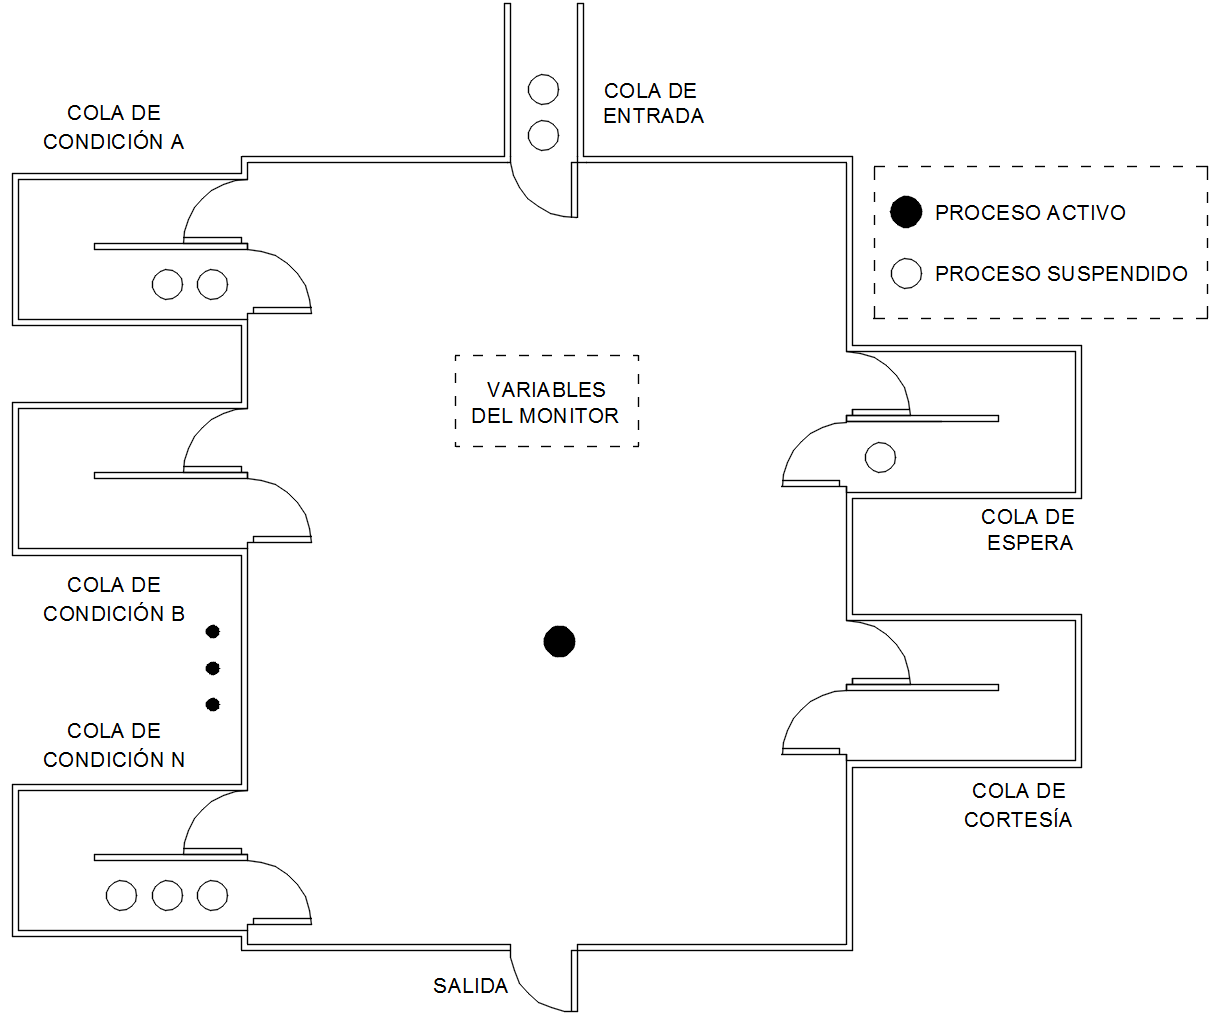
\includegraphics[height=100mm]{Monitor}
  \caption{Estructura de un Monitor de Concurrencia}
  \label{fig:monitor01}
\end{figure}

\paragraph{Cola de cortesía:}
Cuando un proceso libera a otro de mayor prioridad, tiene la opción de cederle
su lugar en el monitor. Si decide hacer esto, debe esperar fuera del monitor
para luego reanudar su ejecición dentro del mismo. Un posible lugar donde hacer
esta espera es la \textit{cola de cortesía}.
La cola de cortesía es una cola de espera que no está atada a ninguna condición.
Un proceso debería llamar a $signal$ sobre esta cola en lugar de liberar la
exclusión mutua de entrada si existe algún proceso esperando allí.

En la figura \ref{fig:monitor_cortesia} se observa la estructura de un monitor
con cola de cortesía.

\begin{figure}[h]
  \centering
  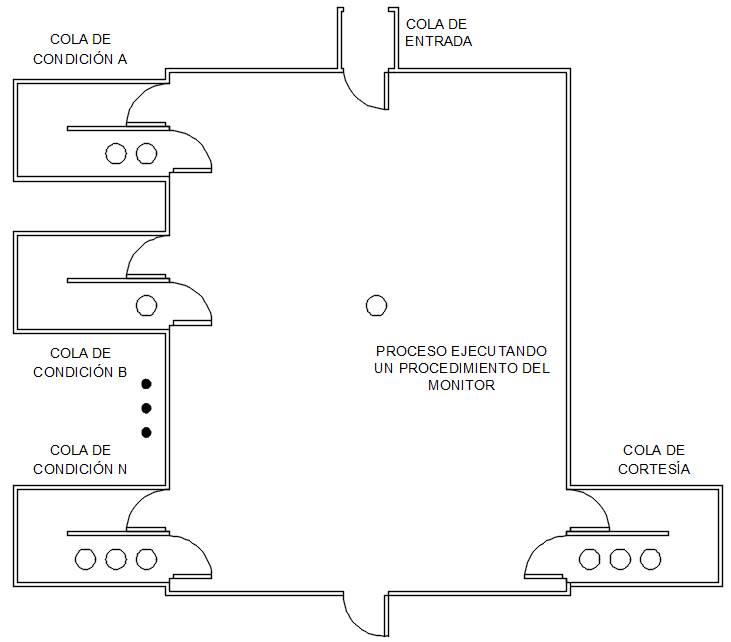
\includegraphics[height=100mm]{Monitor_Cortesia}
  \caption{Estructura de un Monitor de Concurrencia con Cola de Cortesía}
  \label{fig:monitor_cortesia}
\end{figure}

\subsubsection{Políticas de desbloqueo en monitores}
\label{politica_monitor}
El desbloqueo de un hilo suspendido por una llamada a $delay(X)$ sobre la
condición $X$ debe ser hecha por el hilo que produjo el cambio en la condición
$X$. Al analizar esta situación se desprenden múltiples formas de realizar esta
operación.

Para todos los siguientes casos, se considera que el proceso \textit{A}
desbloquea al proceso \textit{B} ejecutando $signal(x)$, condición sobre la que
\textit{B} se encuentra bloqueado inicialmente.

\paragraph{Desbloquear y continuar}
\textit{A} desbloquea a \textit{B} y continúa su ejecución dentro del monitor,
ya sea hasta terminar la llamada al procedimiento o hasta bloquearse en una cola
de condición. Una vez \textit{A} sale del monitor, \textit{B} ejecuta la
instrucción siguiente al $delay(x)$ que lo bloqueó.
En este punto, \textit{B} debe volver a verificar la condición que lo suspendió
porque no se puede garantizar que \textit{A} no la haya modificado luego de la
llamada a $signal(x)$.

\paragraph{Retorno forzado}
\textit{A} ejecuta una instrucción de salida del monitor ($return$ o $delay(n)$)
justo después de desbloquear a \textit{B}.
De esta manera, no es necesario que \textit{B} vuelva a comprobar su condición
ya que la exclusión mutua asegura que no fue modificada.

\paragraph{Desbloquear y esperar}
\textit{A} desbloquea a \textit{B} y automáticamente se agrega a la cola de
entrada del monitor.
Este enfoque tiene la ventaja de que \textit{B} no necesita comprobar su
condición de bloqueo una vez desbloqueado, pero \textit{A} cede su lugar en el
monitor y debe volver a competir por el ingreso para poder terminar su
ejecución.

\paragraph{Desbloquear y espera urgente}
Esta política soluciona el problema de inequidad de \textit{Desbloquear y
esperar}. Luego de desbloquear a \textit{B}, \textit{A} le cede su lugar en el
monitor, aunque en lugar de suspenderse en la cola de entrada del monitor lo
hace en la \textit{cola de cortesía}. De esta manera, el desbloqueo de
\textit{A} tendrá prioridad sobre el de cualquier proceso que intente entrar al
monitor.

\paragraph{Conclusión:}
Como con los semáforos, es posible cometer errores en la sincronización de los
monitores. La ventaja que tienen los monitores sobre los semáforos es que todas
las funciones de sincronización están confinadas dentro del monitor. De este
modo, es sencillo verificar que la sincronización se ha realizado correctamente
y detectar los fallos. Es más, una vez que un monitor está correctamente
programado, el acceso al recurso protegido es correcto para todos los procesos.
Con los semáforos, en cambio, el acceso al recurso es correcto sólo si
\textbf{todos los procesos} que acceden al recurso están correctamente
programados.\cite{SistOpStallings}
Por otro lado, las políticas de desbloqueo permiten especificar prioridades de
ejecución para los hilos, priorizando ya sea por orden de llegada o por algún
otro criterio. Si a su vez, se construye el monitor de forma modular para
cambiar la política de manera simple, se puede alterar la planificación de los
hilos de acuerdo a cada caso, según sea necesario. Si esto se intenta hacer
utilizando semáforos, resultaría mucho más difícil.


    \part{Desarrollo}
        \chapter{Investigación}
            \section{Requerimientos}

\begin{enumerate}
	\item El sistema debe delegar flujo de ejecución a un motor de
	petri.
	\begin{itemize}
		\item El sistema debe mapear transiciones de una red de petri a eventos
		especificados por los usuarios. Un evento puede ser equivalente a un conjunto de transiciones.
		\item Cuando un evento es desencadenado por el disparo de un conjunto de
		transiciones el sistema debe ejecutar todas las tareas que se encuentran registradas al evento.
		\item Cuando un suceso definido por el usuario ocurre, el sistema debe
		notificar todos los eventos asociados a este suceso al motor de petri.
		\item El sistema debe proveer una interface para que el usuario pueda
		suscribir sucesos, tareas y fines de tareas a eventos especificados por el usuario.
		\item El sistema debe proveer una interface para que el usuario pueda definir
		eventos.
		\item Cuando una tarea termina el sistema debe notificar al motor de petri
		acerca de todos los eventos asociados a la finalización de la tarea.
	\end{itemize}
	\item Para un usuario con conocimiento intermedio en Java y Redes de Petri, el
	framework puede aprender a usarse en una semana o menos.
	\begin{itemize}
	    \item La utilización del sistema puede incorporar como máximo diez
	    conceptos nuevos a aprender por un usuario con un nivel intermedio en Java
	    y redes de Petri.
	    \item El sistema debe ser acompañado con al menos dos ejemplos de uso en
	    los cuales se muestre al menos un 80\% de las funciones del mismo.
	\end{itemize}
	\item El sistema debe ser compatible con las versiones actuales de motores de
	Petri desarrollados en el Laboratorio de Arquitectura de Computadoras de la
	Facultad de Ciencias Exactas y Naturales de la Universidad Nacional de Córdoba.
	\begin{itemize}
	    \item El sistema debe proveer una interfaz para que el usuario ingrese un
	    archivo PNML con la descripción de una red de Petri.
	    \item El sistema puede instanciar un entorno de ejecución de redes de
	    Petri dado que el usuario ha ingresado un archivo PNML conteniendo la
	    descripción de la red y ha elegido el motor de Petri que desea usar.
	    \item El sistema debe utilizar la interface expuesta por el motor de
	    petri.
	\end{itemize}
	\item El sistema quiere tener una interfaz gráfica de usuario para inicializar
	un nuevo proyecto.
	\begin{itemize}
	    \item La interfaz de usuario quiere contener una pantalla 'PNML Loader'
	    	\begin{itemize}
	    	    \item La pantalla debe dejar al usuario buscar en su disco local y
	    	    elegir un archivo.
	    	    \item La pantalla debe dejar al usuario ingresar la dirección a un
	    	    archivo manualmente mediante la escritura con el teclado.
	    	    \item La pantalla debe permitir confirmar la elección de un archivo.
	    	    \item Si el usuario confirma un archivo y el archivo es un PNML válido
	    	    entonces puede usarse para configurar el entorno de ejecución de
	    	    Petri.
	    	    \item Si el usuario confirma un archivo y el archivo no es un PNML
	    	    válido entonces debe mostrarse un error en pantalla y el usuario debe
	    	    ser capaz de elegir otro archivo.
	    	\end{itemize}
	    \item La interfaz de usuario quiere contener una pantalla de creación de
	    eventos
	    \begin{itemize}
	    	    \item La pantalla debe dejar al usuario definir un evento y asociarlo
	    	    con una o más transiciones definidas en un archivo PNML cargado
	    	    previamente por el usuario.
	    	    \item La pantalla de creación de eventos quiere permitir guardar las
	    	    decisiones del usuario en un archivo.
	    	    \item La pantalla de creación de eventos quiere permitir al usuario
	    	    cargar configuraciones a partir de un archivo.
	    	    \item Si un archivo guardado previamente se selecciona para ser
	    	    cargado y su contenido tiene un formato inválido, la pantalla
	    	    quiere mostrar un texto de error especificando el problema y el
	    	    archivo no debe ser cargado.
	    	    \item Si un archivo guardado previamente se selecciona para ser
	    	    cargado y el contenido del archivo contiene uno omás eventos que
	    	    mapean a transiciones inexistentes, la pantalla quiere mostrar un
	    	    texto de error especificando el problema y sólo debe cargarse la
	    	    configuración de los eventos fuera de conflicto.
	    \end{itemize}
	     \item La interfaz de usuario quiere contener una pantalla de selección de
	     el motor de Petri.
	     \begin{itemize}
	         \item La pantalla debe permitir elegir entre un motor de Petri Java,
	         un motor de Petri en hardware o un motor de Petri en driver.
	         \item La pantalla debe comunicar la decisión del usuario para preparar
	         el entorno de ejecución de Petri de acuerdo al motor elegido.
	     \end{itemize}
	         
	\end{itemize}
\end{enumerate}
        \chapter{Monitor de Concurrencia con Redes de Petri}
            \section{Introduccion}

Como se dijo en la sección [{\color{red}CITAR OBJETIVOS DONDE SE QUIERE
SEPARAR LA LÓGICA DEL CÓDIGO EJECUTANDO EL MODELO}], uno de los objetivos de
este proyecto integrador es modelar sistemas reactivos para garantizar su
correcto diseño.
Para esto se propone modelar el sistema con RdP (ver sección \ref{redes_de_petri}).
Otro objetivo planteado es separar la lógica de un sistema del código que
implementa sus funcionalidades y su política de gestión de hilos.
Teniendo ambos objetivos es cuenta es que se propone que sea el propio modelo
quien guíe la ejecución lógica del sistema.

Por su naturaleza, los sistemas reactivos son concurrentes y envían y reciben
eventos del mundo exterior.
Por esto se debe hacer una buena gestión de la concurrencia para asegurar su correcto
funcionamiento, utilizando alguna de las técnicas vistas en
la sección \ref{ProgramacionConcurrente} y para modelarlos se debe incluir en
el modelo el envío y recepción de eventos.

Como el modelo de concurrencia obtenido por las RdP es centralizado, resulta
casi natural ejecutar una RdP como lógica secuencial de un sistema reactivo
dentro de un monitor de concurrencia. Luego, para relacionar los eventos con el
monitor se utilizan RdP no autónomas.

\section{\javapetriconcurrencymonitor}

\javapetriconcurrencymonitor es un monitor de concurrencia que ejecuta Redes
de Petri, hecho en lenguaje de programación Java.
Provee al usuario de una interfaz de programación de aplicaciones (API) para
ejecutar una RdP, pretegiéndola de los problemas de concurrencia con la
exclusion mutua del monitor.

Brinda soporte para:
\begin{itemize}
  \item Redes de Petri:
  \begin{itemize}
    \item Plaza-Transición
    \item Temporales
  \end{itemize}
  
  \item Tipos de arcos;
  \begin{itemize}
    \item Normal
    \item Lector o de Prueba
    \item Inhibidor
    \item Reset
  \end{itemize}
  
  \item Carga de RdP en lenguaje PNML (dialecto de TINA)
  \item Guardas
  \item Transitiones automáticas
  \item Subscripción a eventos en transiciones informadas
  \item Políticas intercambiables y extensibles de prioridad de disparo
  \item Disparos perennes y no-perennes

\end{itemize}

        \chapter{\nombreFramework \  Framework}
            \section{Fundamentos del Framework}
En la sección~\ref{sec:petri_concurrency_monitor_intro} se propone utilizar RdP
como la lógica secuencial de un sistema concurrente. Para logralo, se
implementó el monitor de petri por software descripto en la
sección~\ref{sec:java_petri_concurrency_monitor}.
Este monitor permite delegar la concurrencia y asincronismo del
sistema a una red de Petri \cite{TesisMicolini}. Un ejemplo de uso exitoso se
describe en \cite{Bentivegna-Ludemann}.

La utilización directa del monitor es engorrosa y genera un
alto grado de acoplamiento entre el software de usuario y la red de Petri
puesto que los eventos de la red quedan asociados directamente a los eventos del
mundo real que modela.
La principal desventaja de un sistema acoplado a la red de Petri está dada por la
reducción de la escalabilidad del sistema. Esto se debe a que una modificación
de la lógica, que conlleva una sustitución de la red, implica también un cambio
en el código del software. En consecuencia, dificulta el proceso de desarrollo y
su mantenibilidad. Otra desventaja es que impide la reutilización de redes de
Petri genéricas, útiles para resolver diferentes problemas de
características similares.

Un requerimiento importante de este proyecto consiste en la facilidad de uso.
Como se explicó en el párrafo anterior, la utilización del monitor en forma
directa presenta una complejidad elevada y favorece a la generación de errores,
ya que deben crearse todos los hilos de ejecución y deben programarse los disparos de
transición de forma manual en el código. Este problema se manifiesta, por
ejemplo, en soluciones como CodeGen \cite{codegen}.
Ante un cambio en la Red de Petri deben modificarse algunos o todos los
disparos de transición distribuidos a lo largo del código. En caso de un error
en esta tarea, se genera una sincronización incorrecta de los hilos.

A su vez, para desacoplar las acciones que debe realizar el sistema de los
eventos, es necesario incorporar una entidad encargada de manejar y ejecutar
dichas acciones.

Como resultado de este análisis, se llegó a la conclusión de que es necesario
embeber el monitor de Petri en un framework que se encargue de desacoplar el
código de usuario de la lógica de disparos.
Una conclusión de similares características se desprende de
\cite{Bentivegna-Ludemann}, donde los autores expresan: ``La debilidad
encontrada en el proceso de elaboración del software, es que resultó
problemático vincular los hilos con las transiciones de la RdP. Esto se debe a
que entre las acciones y las transiciones no existe una capa de abstracción
para mapear las mismas.
Por lo cual, queda en evidencia que es necesaria la existencia de un framework
para automatizar y facilitar la vinculación entre eventos, acciones y
transiciones.''


\section{Sincronización por Red de Petri a través de Eventos}
\label{sec:sincronizacion_RdP_por_eventos}
Los sistemas a desarrollar utilizando el monitor descripto en la
sección~\ref{sec:java_petri_concurrency_monitor}, son programas de software que
intercambian eventos con la red de Petri y con su entorno físico.

\begin{figure}[h]
	\centering
	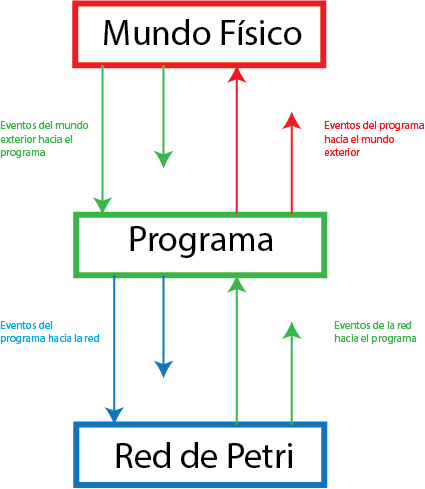
\includegraphics[width=75mm]{eventos_petri-programa-mundo}
	\caption{Intercambio de eventos en un programa sincronizado por Red de Petri}
	\label{fig:eventos_petri-programa-mundo}
\end{figure}

El programa tiene la posibilidad de acceder a hardware del mundo físico, ya sea
para realizar una acción (por ejemplo utilizando actuadores) o  para obtener
eventos del mundo exterior y comunicarlos a la red de Petri (por ejemplo con
sensores).

La red toma los eventos del mundo exterior y, dependiendo de las condiciones del
problema y del estado global, calcula los eventos hacia el programa.
La red es un procesador de eventos. \cite{TesisMicolini}\cite{chimp}

Este concepto se amplía en la sección Eventos Físicos y Eventos
Lógicos de \cite{chimp}. En esta sección se distingue la existencia de los dos
tipos de eventos mencionados, y se los define como:
  \begin{itemize}
    \item Eventos Lógicos: eventos que son comprensibles por el monitor de
    redes de Petri, y están inherentemente asociados a transiciones de la red
    misma y sus colas.
    \item Eventos Físicos: suceden en el mundo físico y representan sucesos del
    dominio del problema. Están conectados con el software.
  \end{itemize}

Tras la incorporación del concepto de eventos lógicos y físicos, en \cite{chimp}
se propone un diagrama de arquitectura de alto nivel como el de la
Figura~\ref{fig:eventos_fisicos-logicos}.

\begin{figure}[h]
	\centering
	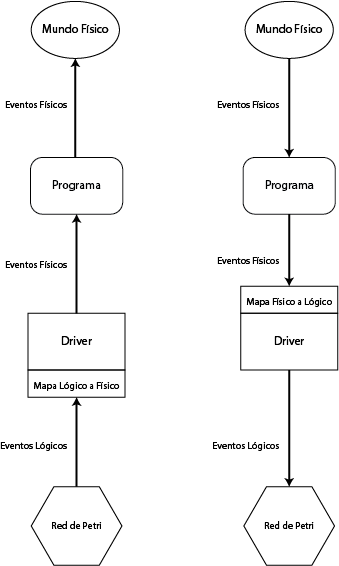
\includegraphics[width=75mm]{eventos_fisicos-logicos}
	\caption{Arquitectura con Eventos Físicos y Lógicos}
	\label{fig:eventos_fisicos-logicos}
\end{figure}

Los eventos físicos representados en la
Figura~\ref{fig:eventos_fisicos-logicos} abarcan dos tipos de eventos. Uno de
ellos está efectivamente relacionado con el hardware o software externos al
sistema (mundo físico). El otro tipo de eventos está relacionado con el manejo
de las acciones que van a realizar dichos elementos del mundo exterior, el cual
se ejecuta a través del software del sistema.
Por este motivo se determinó que la clasificación de los
eventos en dos tipos no es suficiente para explicar la comunicación en un
sistema de estas características. 

A partir de lo expuesto en el párrafo previo, se modifica la clasificación
de eventos existente:

\begin{itemize}
    \item Eventos Lógicos: Conserva la definición descripta previamente. Este
    tipo de eventos se comunica utilizando las interfaces proporcionadas por el
    monitor de redes de Petri.
    \item Eventos Físicos: suceden en el mundo físico y representan sucesos del
    dominio del problema. Este tipo de eventos se comunican a través de las
    interfaces que expone el elemento del mundo exterior y las interfaces que
    ofrece el lenguaje de programación utilizado para desarrollar el software.
    Por ejemplo pueden comunicarse a través de Event Listeners, mecanismos
    de IPC, Sockets, Serial, Bluetooth, etc.
    \item Eventos de Acción: Evento intermedio
    entre los eventos físicos y lógicos. Este tipo de eventos es manejado
    por el framework durante la inicialización del sistema. Cumplen una función
    de abstracción entre las acciones de software y los eventos lógicos,
    necesaria para desacoplar la red de Petri del software y permitir la
    inversión de control descripta en la sección~\ref{sec:inversion_control}.
\end{itemize}

A partir de la nueva clasificación de los eventos del sistema emerge una nueva
arquitectura de alto nivel. A su vez emergen nuevos requerimientos, relacionados
con el requerimiento número 2 de la sección~\ref{sec:definicion_reqs}. A continuación
se listan los nuevos requerimientos:

\begin{itemize}
  \item El monitor de RdP debe manejar los eventos lógicos del sistema,
  mediante las interfaces de disparo y seteo de guardas.
  \item El framework debe ofrecer interfaces para mapear eventos lógicos de una
  RdP a eventos de acción especificados por los usuarios.
\end{itemize}

\subsection{Arquitectura de alto nivel de \nombreFramework}
\label{sec:arquitectura_alto_nivel}
Un sistema informático consiste en una secuencia de acciones que se ejecutan
ante el cumplimiento de determinadas condiciones. Desde el punto de vista del
programa que analiza dichas condiciones, se las clasifica en síncronas y asíncronas.
  \begin{itemize}
	\item Síncronas: Están sicronizadas con la ejecución del programa. Se
	desencadenan en un momento específico, conocido de antemano.
	Por ejemplo, condiciones booleanas derivadas del estado del sistema que
	realizan cambios en el flujo de instrucciones del mismo (saltos
	condicionales).
	\item Asíncronas: Se desencadenan en cualquier momento, de forma independiente
	a la ejecución del programa. Por ejemplo, eventos provenientes del mundo
	exterior o mensajes entre procesos.
  \end{itemize}

El objetivo de este trabajo es implementar un framework dirigido por redes de
Petri para controlar la ejecución de todas aquellas acciones que respondan a
estos tipos de condiciones.
De esta forma, será el monitor de redes de Petri quien analice las condiciones y
explicite el estado del sistema. Así, es responsabilidad de la red:
\begin{itemize}
  \item Disparo de eventos provenientes de sistemas externos, que pueden llegar
  en cualquier instante de tiempo y sin un orden preestablecido. Los estados
  locales de la red se mantienen en causalidad de las acciones ejecutadas con
  anterioridad. El monitor es el encargado de mantener el estado lógico del
  sistema.
  
  \item Condiciones de sincronización para el ordenamiento de la ejecución de
  acciones en el tiempo. 
  
  \item Condiciones impuestas por el dominio del problema. El monitor es el
  encargado de impedir la ejecución de una acción hasta que la misma pueda ser
  realizada sin riesgos.
\end{itemize}

De acuerdo a lo estudiado en la sección~\ref{sec:inversion_control}, una
característica principal de un framework es la inversión de control. Por este
motivo, el diseño de la arquitectura del framework contempla el control del
flujo de ejecución del código de usuario.

\begin{figure}[H]
	\centering
	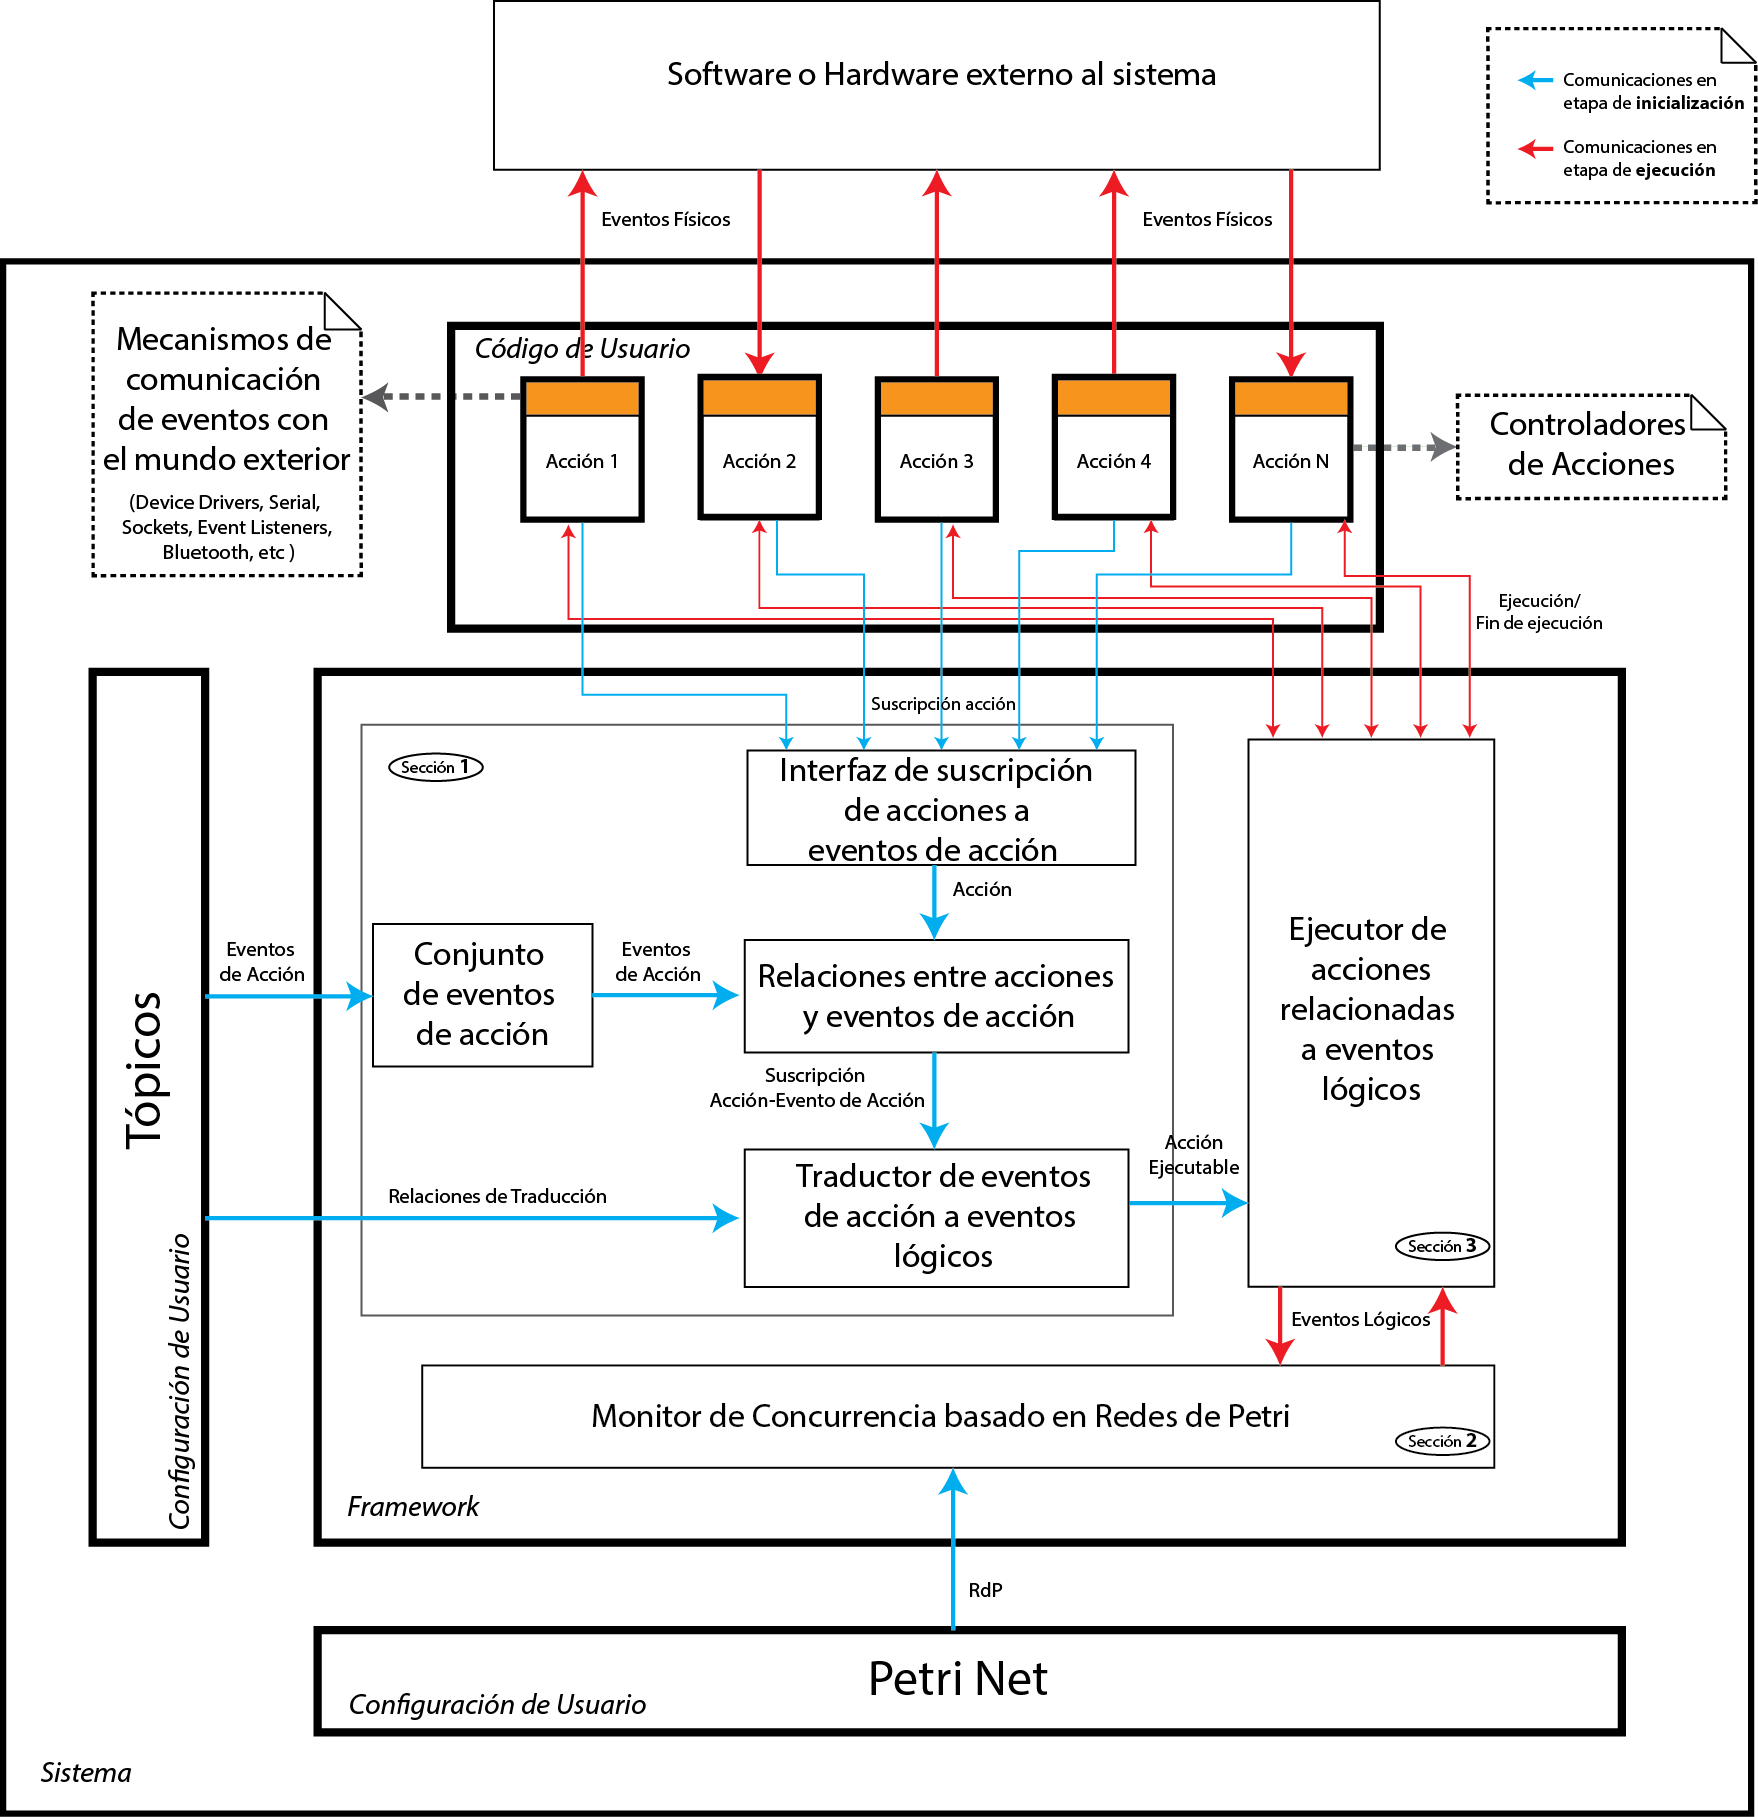
\includegraphics[width=0.9\textwidth]{arquitectura_framework}
	\caption{Diagrama de Arquitectura de Alto Nivel}
	\label{fig:arquitectura_petri-manejador-acciones-mundo}
\end{figure}

Como puede apreciarse en la
Figura~\ref{fig:arquitectura_petri-manejador-acciones-mundo}, \nombreFramework
Framework puede dividirse en tres partes a nivel de arquitectura:
\begin{enumerate}
  \item Un conjunto de módulos para la suscripción a eventos de acción (ver
  sección 1) encargado de:
  \begin{itemize}
    \item Ofrecer interfaces para definir los eventos de acción del sistema.
    \item Ofrecer interfaces para suscribir las acciones del sistema a los
    eventos de acción correspondientes.
    \item Ofrecer interfaces para definir las reglas de traducción entre eventos
    de acción y eventos lógicos.
    \item Encapsular las acciones junto a los eventos lógicos necesarios para su
    sincronización.
  \end{itemize}
\item Un monitor de redes de Petri (ver sección 2) cuyas responsabilidades son:
	\begin{itemize}
	  \item Brindar las interfaces para la incorporación del modelo de Red de Petri
	  del sistema, el cual contiene la definición de los eventos
	  lógicos.
	  \item Garantizar el cumplimiento de las condiciones de sincronización y
	  exclusión mutua de la concatenación de acciones.
	\end{itemize}
\item Un sistema ejecutor de las acciones definidas por el usuario (ver sección 3). 
  Se encarga de:
  \begin{itemize}
	  \item Intercambiar eventos lógicos con el monitor para asegurar la
	  sincronización y exclusión mutua en la ejecución de las acciones.
	  \item Ejecutar las acciones cuando las condiciones de ejecución
	  estén dadas.
	  \item Intercambiar eventos lógicos con el monitor para informar acerca de la
	  finalización de la ejecución de una acción.
	\end{itemize}
\end{enumerate}

Por su parte, el programa de usuario puede dividirse en:
\begin{enumerate}
  \item Una Red de Petri conteniendo el modelo de la lógica del sistema.
  \item Tópicos que contienen la definición de los eventos de acción y sus
  reglas de traducción a eventos lógicos.
  \item El código de usuario. Contiene todas las acciones de software
	concretas a realizar, con sus correspondientes suscripciones a eventos
	de acción. Dichas acciones pueden comunicarse con el mundo exterior. Por esta
	razón, \textbf{\emph{el manejo de los eventos físicos es responsabilidad del
	usuario}}.
\end{enumerate}

\begin{framed}
\textbf{Notas:} 
\begin{itemize}
\item Los controladores de acciones se ejecutan cuando el monitor de red de
Petri lo dispone. El monitor es el encargado de bloquear o liberar los hilos de una
acción de acuerdo a las condiciones de sincronizacion. Por otro lado, cuando una
acción finaliza, el sistema de ejecución se encarga de dar aviso al monitor.

\item La definición y el desarrollo de las acciones de software, y su
asociación a los eventos de acción correspondientes quedan a cargo del usuario
desarrollador. 

\item El usuario no decide en qué momento se ejecuta la acción, ya que
con el fin de lograr la inversión de control, dicha responsabilidad es otorgada
al monitor de redes de Petri.
\end{itemize}
\end{framed}
            \section{Modos de Sincronización de Acciones utilizando Redes de Petri}
\label{sec:sincronizacion_cinta_transportadora}
En esta sección se analizan dos formas de llevar la sincronización de las
acciones mediante la utilización de las interfaces proporcionadas por el monitor
de Redes de Petri. Estos modos se denominan:
\begin{enumerate}
  \item Sincronización por aviso de ejecución.
  \item Sincronización por petición de ejecución.
\end{enumerate}

Para estudiar los modos de sincronización mencionados se hará uso de un caso de
ejemplo, descripto a continuación:

\begin{labeling}{description}
\item [Ejemplo]
Cinta transportadora con 3 estaciones. Se depositan piezas en la primer
estación de manera asincrónica. Cuando esto sucede, la cinta avanza a la
estación 1, donde un operario realiza una transformación a la pieza. Una vez el
operario realizó la transformación, presiona un pulsador y la cinta avanza a la
estación 2, donde el mismo operario empaqueta la pieza. El operario
presiona otro pulsador al finalizar su tarea y luego la cinta avanza una vez
más y la pieza se deposita en un contenedor. Una vez que la pieza llega al
contenedor se habilita el ingreso de una nueva pieza al proceso.
\end{labeling}

\begin{figure}[H]
    \centering
    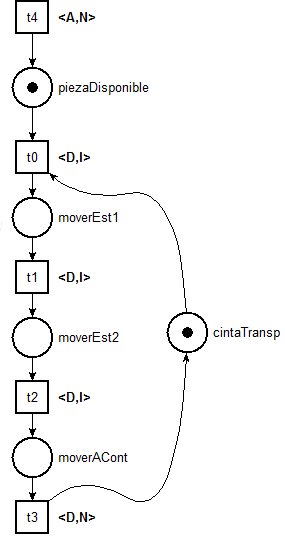
\includegraphics[height=100mm]{Petri_Cinta_Transportadora_1}
    \caption{Red de Petri de una cinta transportadora}
    \label{fig:petri_cinta_transportadora_1}
\end{figure}

\subsection{Análisis de ejecución del caso de estudio, utilizando
sincronización por aviso de ejecución} 
De acuerdo al modo de ejecución por aviso, el monitor recibe eventos desde el
resto del framework, los procesa y luego desencadena la ejecución de las
acciones. A continuación se describe la ejecución del caso de ejemplo siguiendo
el modo de sincronización por aviso de ejecución:
\begin{enumerate}
    \item Debe insertarse un evento en la cola de entrada de
    ``ejecutar\_accion\_1'' cuando la acción que escucha al sensor de pieza
    disponible detecte la llegada de una nueva pieza.
    Si la cinta Transportadora se encuentra disponible, el monitor de petri dispara
    “ejecutar\_accion\_1” y se genera un evento que se deposita en la cola de
    salida de “ejecutar\_accion\_1”.
    \item Un manejador de eventos lee el evento de salida de
    “ejecutar\_accion\_1” y llama a ejecutar la acción “accion\_1”, que mueve
    la pieza a la estación 1 y espera el trabajo del operador. Una vez que el
    operador realiza su trabajo, presiona el pulsador. Esto genera un evento
    que se envía a la cola de entrada de “ejecutar\_accion\_2”. El monitor de
    petri dispara “ejecutar\_accion\_2” y se genera un evento que se deposita
    en la cola de salida de “ejecutar\_accion\_2”.
    \item El manejador de eventos
    lee el evento de salida de “ejecutar\_accion\_2” y llama a ejecutar la
    acción “accion\_2”, que mueve la pieza a la estación 2 y espera el trabajo
    del operador. Una vez que el operador realiza su trabajo, presiona el
    pulsador. Esto genera un evento que se envía a la cola de entrada de
    “ejecutar\_mov\_cont”. El monitor de petri dispara
    “ejecutar\_mov\_cont” y se genera un evento que se deposita en la cola de
    salida de “ejecutar\_mov\_cont”.
    \item El manejador de eventos lee el evento de salida de
    “ejecutar\_mov\_cont” y llama a ejecutar la accion “movimiento\_a\_cont”, que
    mueve la pieza al contenedor. Una vez terminada esa acción envía un evento
    a la cola de entrada de “liberar\_cinta”. El monitor de petri dispara
    “liberar\_cinta” y libera la cinta Transportadora para procesar otra pieza.
\end{enumerate}

A partir del análisis de los pasos de ejecución anteriores, se detectó una
desventaja en este modo de sincronización.
Al utilizar la suscripción a transiciones informadas el módulo
encargado de manejar los eventos provenientes de la Red de Petri asume
una parte del control de la lógica de ejecución del sistema.
De esta manera, el monitor de Redes de Petri delega parte de su
responsabilidad, y se descentraliza el control del sistema. En el caso
particular del framework realizado en~\cite{chimp}, el uso de la sincronización
por avisos de ejecución lleva a que el bloqueo y liberación de hilos se realice
fuera de la estructura del monitor, desaprovechando una de las principales
ventajas de la arquitectura del sistema.
\\

\subsection{Análisis de ejecución del caso de estudio, utilizando
sincronización por petición de ejecución}
\label{sec:sincronizacion_peticion_ejecucion}
 El modo de sincronización por petición de ejecución es un mecanismo de
 sincronización alternativo al modo por aviso de ejecución.
 En este modo, los hilos que ejecutan acciones realizan una petición de
 ejecución al monitor, sin tener en cuenta el estado actual de la red de Petri.
 El monitor es el encargado de bloquear aquellos hilos cuyas acciones no
 pueden ser ejecutadas en el momento de la petición del permiso ejecución. Una
 vez que las condiciones son las adecuadas para realizar la acción, el monitor
 libera al hilo encargado de ejecutarla.
 De esta forma, el manejo de la concurrencia del sistema es realizado
 íntegramente dentro del monitor. El sistema de ejecución basado en
 peticiones es más adecuado para una arquitectura controlada por monitor. 

\begin{enumerate}
    \item Se generan eventos que se encolan en la cola de entrada en
    ``ejecutar\_accion\_1'', ``ejecutar\_accion\_2'', ``ejecutar\_mov\_cont'', y
    ``liberar\_cinta''.
    \item El monitor bloquea los hilos que generaron eventos para
    ``ejecutar\_accion\_2'', ``ejecutar\_mov\_cont'', y ``liberar\_cinta'' por no
    estar sensibilizadas las transiciones en ese momento.
    \item El monitor dispara “ejecutar\_accion\_1”. Y se envía un evento a la
    cola de salida de “ejecutar\_accion\_1”, liberando al hilo bloqueado en
    dicha transición.
    \item El hilo ejecuta la acción “accion\_1”.
    \item Existe un problema, ya que al disparar “ejecutar\_accion\_1”, el
    monitor tiene permitido disparar “ejecutar\_accion\_2”, pero la operación
    “accion\_1” aun no ha finalizado, generando un problema de sincronización.
\end{enumerate}

Dada la red de petri de la Figura~\ref{fig:petri_cinta_transportadora_1}
surgen problemas de sincronización. Por ejemplo, uno de estos problemas
tiene origen al iniciar la acción “accion\_1” cuando existe una petición
de ejecución de la acción “accion\_2”. En este caso el monitor otorga el permiso
de ejecución de “accion\_2” de forma inmediata, sin tener en cuenta si
“accion\_1” ha finalizado.

Del análisis de este caso se desprenden las siguientes conclusiones:
\begin {itemize}
  \item La petición de ejecución permite concentrar el control del flujo de
  	ejecución en el monitor.
  \item Es necesario que el framework dé aviso al
	monitor de un evento de finalización de acción, cuando existen otras partes de
	la red que dependen de este evento.
\end{itemize}

En consecuencia, utilizar un sistema de ejecución basado en peticiones requiere
un nuevo modelo en red de Petri del problema, que sea capaz de sincronizar los
eventos de finalización de acción. A continuación se procede a estudiar tres
formas de sincronizar dichos eventos:
\begin{enumerate}
  \item Evento de finalización de acción por grupo transición-plaza
  \item Evento de finalización de acción por guardas
  \item Evento de finalización de acción por cola de condición de disparo no
  perenne.
\end{enumerate}

\subsubsection{Evento de Finalización de Acción por Grupo
Transición-Plaza}
\label{sec:sincronizacion_peticion_ejecucion_transicion_plaza}
En la Figura~\ref{fig:petri_cinta_transportadora_2} se observa un modelo de
RdP para la sincronización de acciones mediante petición de ejecución, con aviso
de finalización de acción por grupo transición-plaza. Este método consiste en
añadir una transición y una plaza extra por cada acción que
requiera enviar un evento de finalización de acción a la red. Esta transición y
plaza de aviso de finalización deben colocarse en cadena con la plaza que
representa el estado de ejecución de la acción.
\\

\begin{figure}[H]
    \centering
    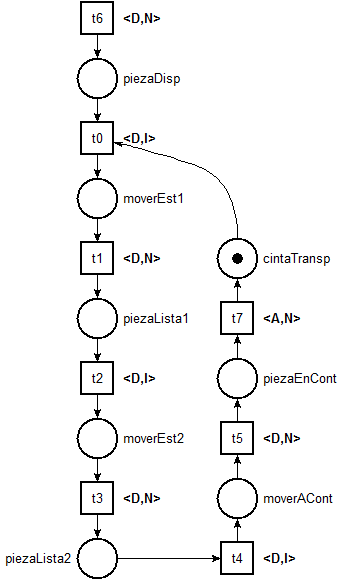
\includegraphics[height=100mm]{Petri_Cinta_Transportadora_2}
    \caption{Red de Petri de una cinta transportadora sincronizada por inserción
    de plaza-transición}
    \label{fig:petri_cinta_transportadora_2}
\end{figure}


A continuación se detalla la ejecución de la red de la
Figura~\ref{fig:petri_cinta_transportadora_2}:\\
\begin{enumerate}
	\item Se generan eventos que se encolan en la cola de entrada en
	``ejecutar\_accion\_1'', ``ejecutar\_accion\_2'', ``ejecutar\_mov\_cont''.
	\item El monitor bloquea los hilos que generaron eventos para
	``ejecutar\_accion\_1'', ``ejecutar\_accion\_2'', ``ejecutar\_mov\_cont''
	por no estar sensibilizadas las transiciones en ese momento.
	\item Llega una pieza y se genera un evento de entrada en “recibir\_pieza”
	\item El monitor dispara “recibir\_pieza” y se coloca un token en “piezaDisp”,
		sensibilizando “ejecutar\_accion\_1”.
	\item El monitor libera el hilo bloqueado en “ejecutar\_accion\_1” ya que ahora tiene permiso
		de ejecución.
	\item Se ejecuta la acción “accion\_1”. Una vez finalizado se genera un evento
	que se envía a la cola de entrada de “finalizar\_acc\_1”.
	\item Como “finalizar\_acc\_1” está sensibilizada el monitor la dispara y se coloca un token
		en “piezaLista1”, sensibilizando “ejecutar\_accion\_2”.
	\item El monitor libera el hilo bloqueado en “ejecutar\_accion\_2” ya que ahora
	tiene permiso de ejecución.
	\item Se ejecuta la acción “accion\_2”. Una vez finalizado se genera un evento
	que se envía a la cola de entrada de “finalizar\_acc\_2”.
	\item Como “finalizar\_acc\_2” está sensibilizada el monitor la dispara y se
	coloca un token en “piezaLista2”, sensibilizando “ejecutar\_mov\_cont”.
	\item El monitor libera el hilo bloqueado en “ejecutar\_mov\_cont” ya que ahora tiene permiso
		de ejecución.
	\item Se ejecuta la acción “movimiento\_a\_cont”. Una vez finalizado se genera
	un evento que se envía a la cola de entrada de “finalizar\_mov\_cont”
	\item Como “finalizar\_mov\_cont” está sensibilizada el monitor la dispara y se coloca un token
		en ``piezaEnCont''.
	\item Se dispara la transición ``liberar\_cinta'', que es automática, y se
	libera el recurso ``cintaTransp''.
\end{enumerate}

La principal ventaja de este método consiste en no modificar la semántica de
la red y no añadir nuevos conceptos ni cambios en la forma de ejecución.
La desventaja más importante es que provoca un incremento considerable de
la cantidad de plazas y transiciones de la red, lo que conlleva el
procesamiento de matrices de mayor tamaño. En la
sección~\ref{sec:complex_sequential_task_controller} se estudia un método que
permiten contrarrestar el aumento de tamaño de la RdP para procesos
secuenciales.

\subsubsection{Evento de Finalización de Acción por Guardas}
En la Figura~\ref{fig:petri_cinta_transportadora_3} se observa un modelo de
RdP para la sincronización de acciones mediante petición de ejecución, con aviso
de finalización de acción por guardas. Este método consiste en la utilización de
una guarda como forma de sincronización entre acciones consecutivas.

\begin{figure}[H]
    \centering
    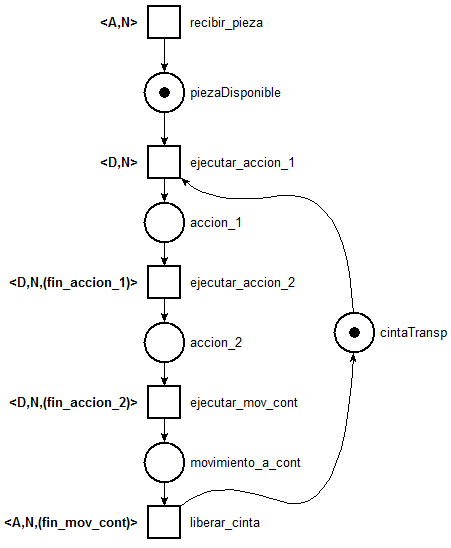
\includegraphics[height=100mm]{Petri_Cinta_Transportadora_3}
    \caption{Red de Petri de una cinta transportadora sincronizada por guardas.}
    \label{fig:petri_cinta_transportadora_3}
\end{figure}

A continuación se detalla la ejecución de la red de la
Figura~\ref{fig:petri_cinta_transportadora_3}
\begin{enumerate}
    \item Se generan eventos que se encolan en la cola de entrada en
    ``ejecutar\_accion\_1'', ``ejecutar\_accion\_2'', ``ejecutar\_mov\_cont''.
	\item El monitor bloquea los hilos que generaron eventos para
	``ejecutar\_accion\_2'' y ``ejecutar\_mov\_cont'' por no estar sensibilizadas
	las transiciones en ese momento.
	\item Se dispara ``ejecutar\_accion\_1'' y se coloca un token en ``accion\_1''.
	Comienza la ejecución de la acción ``accion\_1''. La transición
	``ejecutar\_accion\_2' no se encuentra sensibilizada dado que la guarda
	``fin\_accion\_1'' tiene estado ``false''.
	\item Finaliza la ejecución de ``accion\_1'' y se establece la guarda
	``fin\_accion\_1'' con estado ``true''.
	\item Al estar sensibilizada ``ejecutar\_accion\_2'', se dispara y se libera el hilo
	bloqueado en su cola de condición. Se coloca un token en ``accion\_2'' y
	comienza la ejecución de esta acción. La transición ``ejecutar\_mov\_cont'' no
	se encuentra sensibilizada dado que la guarda ``fin\_accion\_2'' tiene estado
	``false''.
	Se establece la guarda ``fin\_accion\_1'' a ``false'' nuevamente.
	\item Finaliza la ejecución de ``accion\_2'' y se establece la guarda
	``fin\_accion\_2'' con estado ``true''.
	\item Al estar sensibilizada ``ejecutar\_mov\_cont'', se dispara y se libera
	el hilo bloqueado en su cola de condición. Se coloca un token en
	``movimiento\_a\_cont'' y comienza la ejecución de esta acción. La transición
	``liberar\_cinta'' no se encuentra sensibilizada dado que la guarda
	``fin\_mov\_cont'' tiene estado ``false''.
	Se establece la guarda ``fin\_accion\_1'' a ``false'' nuevamente.
	\item Finaliza la ejecución de ``movimiento\_a\_cont'' y se establece la guarda
	``fin\_mov\_cont'' con estado ``true''.
	\item Al estar sensibilidada, se dispara la transición ``liberar\_cinta'', que es
	automática, y se libera el recurso ``cintaTransp''. Se establece la guarda
	``fin\_mov\_cont'' a ``false'' nuevamente.
\end{enumerate}

La ventaja de este método es que permite resolver el problema de sincronización
sin aumentar la cantidad de componentes de la red de Petri.
Como desventaja se puede mencionar que el diseño
del monitor de petri soporta una única guarda por transición, por lo tanto esta
solución impide la utilización de la guarda para otros propósitos. Otra
desventaja importante de la utilización de guardas es que al ser un valor
binario, lleva a una pérdida de eventos de finalización cuando
múltiples hilos realizan una misma acción.

Con el fin de ejemplificar la pérdida de eventos de finalización al utilizar
sincronización de finalización de acción por guardas se analiza el siguiente
caso de ejemplo:
\begin{labeling}{description}
\item [Ejemplo]
	Una ``tarea A'' es realizada por multiples hilos de manera independiente, y cada
	hilo realiza la ``tarea A'' en su totalidad. A su vez una ``tarea B'', que
	debe realizarse luego de la finalización de la ``tarea A'', es ejecutada por
	un único hilo. En este caso la utilización de guardas podría llevar a una
	pérdida de eventos de finalización de la ``tarea A'' debido a la condición
	binaria de la guarda. En la red de la Figura
	~\ref{fig:ejecucion_multiples_hilos_guardas}, un máximo de 5 hilos puede
	ejecutar la ``tarea A'' al mismo tiempo. En el estado que muestra la
	figura existen tres hilos corriendo la ``tarea A''. De acuerdo al planteo de
	este problema, la ``tarea B'' es ejecutada por un único hilo. Cuando dos o más
	hilos finalizan la ``tarea A'' y establecen la guarda ``Fin\_TareaA'' en ``true'',
	existe la posibilidad de que otro hilo dispare ``t1'' antes de comenzar la
	ejecución de la ``tareaB''. En este momento, el hilo que dispara ``t1''
	modifica el valor de la guarda ``Fin\_TareaA'' a ``false'', sobreescribiendo
	el aviso de finalización de acción de los hilos que ya habían establecido
	``Fin\_TareaA'' en ``true''. De esta manera, se pierden eventos de aviso de fin
	de ejecución, provocando la incorrecta sincronización del sistema.
\end{labeling}

\begin{figure}[H]
    \centering
    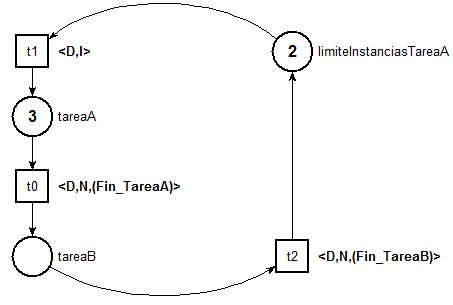
\includegraphics[height=60mm]{Ejecucion_Tarea_Multiples_Hilos_Guardas}
    \caption{RdP: Problema de sincronización de acciones dependientes usando
    guardas, debido a su condición binaria}
    \label{fig:ejecucion_multiples_hilos_guardas}
\end{figure}


\subsubsection{Evento de Finalización de Acción por Cola de Condición de
Disparo No Perenne}
En la Figura~\ref{fig:petri_cinta_transportadora_4} se observa un modelo de
RdP para la sincronización de acciones mediante petición de ejecución, con aviso
de finalización de acción por cola de condición de disparo no perenne. 
Esta forma de solucionar la sincronización de acciones dependientes
supone añadir una nueva propiedad ``P'' a las transiciones. Los hilos
bloqueados en la cola de condición de una transición con propiedad ``P'' sólo
se liberan cuando la transición se encuentra habilitada y además un hilo
externo realiza un disparo no perenne sobre la transición.

\begin{figure}[H]
    \centering
    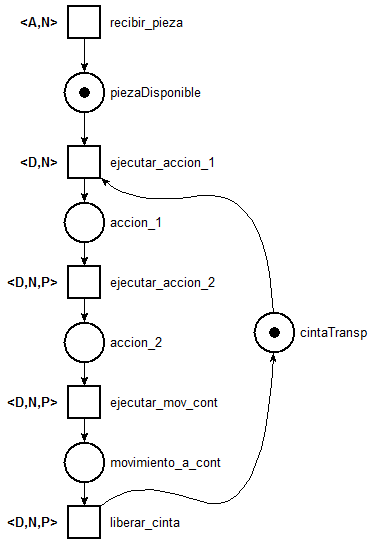
\includegraphics[height=100mm]{Petri_Cinta_Transportadora_4}
    \caption{Red de Petri de una cinta transportadora sincronizada por
    propiedad ``P''.}
    \label{fig:petri_cinta_transportadora_4}
\end{figure}

\begin{enumerate}
    \item Se generan eventos que se encolan en la cola de entrada en
    ``ejecutar\_accion\_1'', ``ejecutar\_accion\_2'', ``ejecutar\_mov\_cont'',
    y ``liberar\_cinta''.
	\item El monitor bloquea los hilos que generaron eventos para
	``ejecutar\_accion\_2'', ``ejecutar\_mov\_cont'', y ``liberar\_cinta'' por
	no estar sensibilizadas las transiciones en ese momento.
	\item Se dispara ``ejecutar\_accion\_1' y se coloca un token en ``moverEst1''.
	Comienza la ejecución de la acción ``accion\_1''. La transición
	``ejecutar\_accion\_2'' no se dispara ya que es de tipo ``P''.
	\item Finaliza la ejecución de ``accion\_1'' y un hilo dispara 
	``ejecutar\_accion\_2'' de forma no perenne para dar aviso de la finalización
	de la acción.
	\item Se libera el hilo bloqueado en cola de condición de
	``ejecutar\_accion\_2''. Se coloca un token en ``accion\_2'' y comienza la
	ejecución de esta acción. La transición ``ejecutar\_mov\_cont'' no se dispara
	ya que es de tipo ``P''.
	\item Finaliza la ejecución de ``accion\_2'' y un hilo dispara
	``ejecutar\_mov\_cont'' de forma no perenne para dar aviso de la finalización
	de la acción.
	\item  Se libera el hilo bloqueado en cola de condición de
	``ejecutar\_mov\_cont''. Se coloca un token en ``movimiento\_a\_cont'' y
	comienza la ejecución de esta acción. La transición ``liberar\_cinta'' no se dispara ya
	que es de tipo ``P''.
	\item Finaliza la ejecución de ``movimiento\_a\_cont'' y un hilo dispara
	``liberar\_cinta'' de forma no perenne para dar aviso de la finalización de la
	acción.
	\item Se libera el recurso ``cintaTransp''.
\end{enumerate}

La ventaja de esta solución es que no incrementa el numero de componentes de la
red. Su principal desventaja consiste en que añade una nueva etiqueta a la
RdP, dificultando su validación matemática. Esta solución supone añadir
una interfaz al monitor de Petri para bloquear hilos en una cola de condición de
una transición tipo P y que los hilos bloqueados en esta cola de condición sólo
puedan liberarse por medio de un disparo no perenne ocasionado por un hilo
externo.
El hilo que realiza el disparo sobre la transición debe realizar una operación
\emph{release} sobre la cola de condición de disparos no perennes (sin importar
si existen o no hilos bloqueados en la cola) para evitar la pérdida de eventos de
finalización de acción.

\subsection{Resumen de Modos de Sincronización}
\label{sec:resumen_sincronizacion}
Existen dos maneras de coordinar la ejecución de las acciones a partir de una
red de Petri.\\ 
\begin{enumerate}
  \item \textbf{Sincronización por aviso de ejecución: } Consiste en suscribir
  una acción a una transición, que envía una notificación en el momento en que
  es disparada. Ante un informe de esta transición, la acción suscripta
  comienza su ejecución.
  Al finalizar una acción, se dispara la transición a la cual está suscripta la
  siguiente acción a ejecutar.
  La principal desventaja de este método consiste en la descentralización del
  manejo de los hilos por parte del monitor, lo cual va en contra de los objetivos del
  proyecto.
  \item \textbf{Sincronización por petición de ejecución: } Los hilos que
  ejecutan acciones realizan una peticion de ejecución al monitor (mediante el
  disparo de transiciones), sin tener en cuenta el estado actual de la red de
  Petri. De este modo el monitor bloquea los hilos que no pueden ejecutarse y
  libera los hilos que cumplan con las condiciones de ejecución. El manejo de
  la concurrencia es llevado a cabo íntegramente por el monitor.
  Para sincronizar acciones dependientes entre sí (una debe comenzar luego de
  la finalización de la otra) se requiere un modo de dar aviso al monitor de
  la finalización de una acción. Se analizan tres opciones:
  \begin{itemize}
      \item Evento de finalización de acción por grupo transición-plaza
	  \item Evento de finalización de acción por guardas
	  \item Evento de finalización de acción por cola de condición de disparo no
	  perenne.
  \end{itemize}
  Se optó por adoptar el evento de finalización de acción por grupo
  transición-plaza. Esta forma presenta la ventaja de no añadir
  conceptos nuevos a la RdP, facilitando el entendimiento de la misma. Además
  no presenta pérdida de eventos de finalización de acción.
  La principal desventaja del grupo transición-plaza consiste en el incremento
  del tamaño de la RdP. En procesos secuenciales, puede contrarrestarse mediante
  el uso del controlador de acciones descripto en la
  sección~\ref{sec:complex_sequential_task_controller}.
\end{enumerate}
 

 
 
 
 

            \section{Clasificación de Eventos Físicos: \\Eventos Task y Eventos Happening}
\label{sec:clasificacion_eventos_fisicos} 
Se realizó un análisis de los eventos físicos de entrada y los eventos
físicos de salida para determinar su relación con la red de Petri. Se
observa que una acción que emite un evento físico de salida es desencadenada,
en primera instancia, por decisiones tomadas unilateralmente dentro del monitor
de Petri, dependendiendo exclusivamente del estado actual de la red. En cambio,
una acción que se encarga de recibir y manejar un evento físico de entrada depende de la
ocurrencia de dicho evento en el mundo exterior y de la sincronización
realizada por el monitor, dependendiendo del estado actual de la red.
\emph{\color{red} AGREGAR IMAGEN explicativa usando redes de petri y acciones}

Desde este punto de vista, se decidió dar una clasificación más significativa a
los eventos físicos. Esta clasificación estará presente a lo largo de todo
el desarrollo del framework.
\begin{itemize}
  \item Eventos Task (Tarea): Eventos físicos de salida. Son
  desencadenados y sincronizados exclusivamente por eventos lógicos que dependen
  de condiciones ya presentes en el monitor de redes de petri al momento de su
  emisión. Si bien el monitor no produce directamente eventos físicos, puede
  advertirse que un evento task tiene una relación directa con determinados
  eventos lógicos.
  \item Eventos Happening (Suceso): Eventos físicos de entrada. Son
  desencadenados por el mundo externo de manera totalmente asincrónica respecto
  al sistema. La ejecución de las acciones que reciben y manejan estos eventos
  es sincronizada por el monitor de redes de petri. De esta forma, el monitor
  conserva su responsabilidad frente al manejo del asincronismo del sistema.
\end{itemize}

\section{Controladores de Acciones: \\Task Controllers y Happening Controllers}
Las acciones que debe realizar un sistema, junto con los mecanismos de
comunicación de los eventos físicos correspondientes, se encuentran embebidos
dentro de controladores de acción. Los mismos pueden observarse en la
Figura~\ref{fig:arquitectura_petri-manejador-acciones-mundo}. 
Luego de considerar lo expuesto en la
seccion~\ref{sec:clasificacion_eventos:fisicos}, surge la necesidad de
clasificar los controladores de acción respecto a su condición de receptores de
Eventos Happening, o de emisores de Eventos Task. Dicha clasificación
da origen a los controladores de tipo Happening Controller y Task
Controller, respectivamente.

\subsection{Ejecución de un Task Controller}
Haciendo un repaso por algunas características expuestas previamente, se procede
a explicar la ejecución básica de un Task Controller.
De acuerdo a lo expuesto en la sección~\ref{sec:resumen_sincronizacion}, el 
modo de sincronización adoptado es el de petición de ejecución al monitor. 
De esta forma se admiten disparos asíncronos a transiciones realizados desde
diferentes hilos de ejecución, y el monitor se encarga de dormir los hilos que no pueden
ejecutarse.
Otro concepto analizado en la seccion~\ref{sec:clasificacion_eventos_fisicos}
es que un Evento Task tiene una
relacion directa con determinados eventos lógicos. Además, un Evento Task es
desencadenado por condiciones que estan presentes en el monitor al momento de
la emisión de este evento. De esta forma, el comportamiento dinámico de los
Eventos Task será dirigido únicamente por la evolución de los estados de la red
de Petri.

Como corolario del analisis anterior se determina que la ejecución de un Task
Controller puede ser encapsulada en un hilo al momento de inicialización del programa.
Dicho hilo, debe realizar las peticiones de los permisos de sincronización al
monitor de forma directa, sin tener en cuenta el estado de la red. Una vez que
el monitor otorga el permiso, el hilo debe ejecutar el código correspondiente al
Task Controller. Tras la ejecución, el hilo realiza el aviso de finalización al
monitor de Petri.
Estos pasos de ejecución deben repetirse de forma infinita, delegando de esta
forma en el monitor el control de la ejecución del hilo.
La responsabilidad de la creación de los hilos para ejecutar los Task
Controllers pertenece al framework. De esta forma, la ejecución de las
acciones encapsuladas en un Task Controller es transparente al usuario
desarrollador.

\subsection{Ejecución de un Happening Controller}
En la seccion~\ref{sec:clasificacion_eventos_fisicos} se explica que un Evento
Happening se desencadena en el mundo externo y de forma asíncrona al sistema. Es
por ello que un controlador de acción que reacciona ante estos
eventos (Happening Controller) debe ser ejecutado dentro del contexto de un
Listener u Observer del Evento Happening deseado.
Para maximizar las libertades de elección del desarrollador en la recepción de
eventos externos, la responsabilidad de crear estos Listeners se delega en el
usuario. En consecuencia, el código de usuario es quien realiza la llamada a
ejecución de un Happening Controller.
En principio, esto genera un grave problema en cuanto a las responsabilidades
de sincronización.
Las acciones del Happening Controller, al ser ejecutadas en el código de
usuario, quedarían fuera del mecanismo de sincronización del monitor de Petri.
Esto atenta contra el objetivo principal de este trabajo, expuesto en \emph{\color{red} CITA REQUERIDA
objetivo manejo asincronismo}.
Ante esta problemática, se optó por encapsular las instrucciones de
sincronización necesarias dentro de advices de AspectJ que responden a
joinpoints definidos por la ejecución de Happening Controllers.
En consecuencia, cuando el código de usuario hace un llamado a la ejecución del
Happening Controller, la aplicación alcanza un joinpoint. Al alcanzar el
joinpoint se ejecuta el advice dado por la funcion before(), el cual realiza los
pedidos de permiso de sincronización al monitor antes de ejecutar el código del
controller. Una vez que el monitor otorga el permiso, se ejecuta el código del
controller. Al finalizar, se ejecuta el advice dado por la función after(), el
cual realiza los avisos de finalización de ejecución.

En conclusión, la sincronización de la ejecución de los Happening Controllers
sigue siendo una responsabilidad del monitor y es realizada de forma
transparente al usuario. Además, el usuario tiene total libertad para que el
Happening Controller reaccione ante un evento físico de entrada, permitiendo
que la llamada se realice en cualquier punto de la aplicación.






    \bibliography{./bibliografia}
	\bibliographystyle{plain}
\end{document}